%%%%%%%%%%%%%%%%%%%%%%%%%%  phdsymp_sample2e.tex %%%%%%%%%%%%%%%%%%%%%%%%%%%%%%
%% changes for phdsymp.cls marked with !PN
%% except all occ. of phdsymp.sty changed phdsymp.cls
%%%%%%%%%%                                                       %%%%%%%%%%%%%
%%%%%%%%%%    More information: see the header of phdsymp.cls   %%%%%%%%%%%%%
%%%%%%%%%%                                                       %%%%%%%%%%%%%
%%%%%%%%%%%%%%%%%%%%%%%%%%%%%%%%%%%%%%%%%%%%%%%%%%%%%%%%%%%%%%%%%%%%%%%%%%%%%%%


%\documentclass[10pt]{phdsymp} %!PN
\documentclass[twocolumn]{phdsymp} %!PN
%\documentclass[12pt,draft]{phdsymp} %!PN
%\documentstyle[twocolumn]{phdsymp}
%\documentstyle[12pt,twoside,draft]{phdsymp}
%\documentstyle[9pt,twocolumn,technote,twoside]{phdsymp}

\usepackage[english]{babel}       % Voor nederlandstalige hyphenatie (woordsplitsing)

\usepackage{graphicx}			% Om figuren te verwerken.
\graphicspath{{../../../images/}}
\usepackage{booktabs}
\usepackage{times}
\usepackage{siunitx}
\usepackage{xcolor}
\usepackage{amsmath}
\PassOptionsToPackage{hyphens}{url}
\usepackage{hyperref}
\usepackage{url}

\usepackage[acronym,toc,shortcuts]{glossaries}
\setglossarystyle{super}
\renewcommand{\glsnamefont}[1]{\textbf{#1}}
\makeglossaries




%-------------------------------- acroniemen

\newacronym{UABS}{UABS}{Unmanned Arial Base Station}
\newacronym{EIRP}{EIRP}{equivalent isotropic radiation power}
\newacronym{UE}{UE}{User Equipment}
\newacronym{IEC}{IEC}{International Electrotechnical Commission}
\newacronym{SAR}{SAR}{Specific Absorption Rate}
\newacronym{whipp}{WHIPP}{WiCa Heuristic Indoor Propagation Prediction}
\newacronym{DL}{DL}{downlink}
\newacronym{UL}{UL}{uplink}
\newacronym{LTE}{LTE}{Long-Term Evolution}
\newacronym{FDD}{FDD}{Frequency Division Duplex}
\newacronym{TDD}{TDD}{Time Division Duplex}
\newacronym{ICNIRP}{ICNIRP}{International Commission on Non-Ionizing Radiation Protection}
\newacronym{LOS}{LOS}{line of sight}
\newacronym{NLOS}{NLOS}{non line of sight}
\newacronym{Exp Opt}{Exp. Opt.}{exposure optimized}
\newacronym{PwrC Opt}{PwrC. Opt.}{power consuption optimized}
\newacronym{WHO}{WHO}{World Health Organization}
\newacronym{FCC}{FCC}{Federal Communications Commission}
\newacronym{USA}{USA}{United States of America}
\newacronym{IOT}{IoT}{Internet of Things}
\newacronym{UAV}{UAV}{Unmanned Aerial Vehicle}
\newacronym{EU}{EU}{European Union}
%--------------------------------- woordenlijst
\newglossaryentry{isotropicradiator}{
	name = equivalent isotropic radiator,
	text = equivalent isotropic radiator,
	description = A theoretical source of electromagnetic waves which radiates the same intensity for all directions
}

\newglossaryentry{spuriousradiation}{
	name = spurious radiation,
	text = spurious radiation,
	description = According to the thefreedictionary.com: Any emission from a radio transmitter at frequencies outside its frequency band. Also known as spurious emission
}

\newglossaryentry{RRP}{
	name = RRP,
	text = RRP,
	description = RRP is an abreviation used in this paper to indicate an extension on EIRP and stands for Real Radiation Pattern. An RRP value indicates the power (in dBm) for a certain location unlike an EIRP where the power (in dBm) is independent of the location
}

\newglossaryentry{power flux density}{
	name = power flux density,
	text = power flux density,
	description = Magnitude of power ($W$) that travels through a curtain area ($m^2$)
}

\newglossaryentry{thermoregulatory capacity}{
	name = thermoregulatory capacity,
	text = thermoregulatory capacity,
	description = The capacity of an organism to regulate body temperture
}

%\printglossary[type=\acronymtype,title={Lijst van acroniemen}]
%\addcontentsline{toc}{chapter}{\textcolor{maincolor}{Lijst van acroniemen}}
%\printglossary
%\addcontentsline{toc}{chapter}{\textcolor{maincolor}{Verklarende woordenlijst}}






\hyphenation{si-mu-la-ted re-a-lis-tic packets really in-clu-ding}

\def\BibTeX{{\rm B\kern-.05em{\sc i\kern-.025em b}\kern-.08em
    T\kern-.1667em\lower.7ex\hbox{E}\kern-.125emX}}

\newtheorem{theorem}{Theorem}

\begin{document}

\title{	Evaluatie van de elektromagnetische blootstelling van de mens in een netwerk van drones}

\author{Thomas Detemmerman}

\supervisor{Wout Joseph, Luc Martens, Luc Martens, German Dario Castellanos Tache}

\maketitle

\begin{abstract}
De hedendaagse samenleving vertrouwt meer dan ooit op de aanwezigheid van draadloze netwerken. 
Tevens groeit ook de bezorgdheid bij de menigte over de elektromagnetische straling die hierbij gebruikt wordt. De overheid hanteert dan ook
strenge richtlijnen waaraan mobiele toestellen en zendmasten moeten voldoen.

Dit onderzoek tracht de specifieke absorptie snelheid van elektromagnetische straling in kaart te brengen door rekening te houden met alle mobiele 
toestellen en zendmasten. Om dit te verwezelijken wordt gebruik gemaakt van een tool ontwikkeld door de onderzoeksgroep WAVES aan de UGent. Deze tool
simmuleert een volledig netwerk waarbij zendmasten bevestigd worden aan drones. Dit onderzoek observeert verder hoe deze drones kunnen worden aangestuurd
zodoende dat bepaalde doelstellingen zoals het minimaliseren van energieverbruik of elektromagnetische straling bereikt kunnen worden.

Uit de resultaten blijkt dat...
\end{abstract}

\begin{keywords}
LTE, elektromagnetische blootstelling, energieverbruik, drone, femtocell, microstrip patch antenne, stralingspatroon, specifieke absorptietempo (SAT)
\end{keywords}

\section{Introductie}
\PARstart{D}{e} samenleving is meer dan ooit afhankelijk van draadloze communicatie.
Een elektronisch apparaat kan op elk gegeven moment in elke willekeurige plaats beroep doen 
op het draadloze netwerk, gaande van kleine \gls{IOT} apparatuur tot volwaardige zelf-rijdende auto's.

Ook in uitzonderlijke en mogelijks levensbedreigende situaties verwacht de samenleving de aanwezigheid 
van het mobiele netwerk. Desondanks het feit dat dit netwerk zelf mogelijks beschadigd is door de situatie.
Een mogelijk tijdelijke oplossing om een beschadigd network bij te staan is met behulp van onbemande vliegtuigen zoals drones.
Een base station kan geplaatst worden op een drone en zo effici\"ent verplaatst worden naar de nodige locatie.

Deze aanpak is niet alleen handig als het bestaande netwerk beschadigd is maar ook voor onverwachte toename aan gebruikers.
Bijvoorbeeld tijdens de aanslagen op de Brusselse Luchthaven zagen alle mobiele operatoren een toename in data verkeer.
Sommige operatoren raakten zodoende verzadigd dat ze als enige oplossing zagen om de wetgeving te negeren en de 
elektromagnetische straling te laten toenemen zodoende dat toch iedereen behandeld kon worden \cite{baseZaventem}.

De elektromagnetische straling die vrijkomt bij netwerken kunnen echter niet met onachtzaamheid behandeld worden.
Onderzoek toont aan dat buitensporige elektromagnetische straling verscheidinge biologische neveneffecten kunnen veroorzaken \cite{bioeffects,WHO}.
Het wordt dus duidelijk dat elektromagnetische straling een sleutelrol speelt bij het ontwikkelen van een met drones beholpen netwerk 
waarbij de wetgeving nauwkeurig nageleefd dient te worden.

Drone-gestuurde netwerken kunnen dankzij hun mobiliteit eenvoudig verplaatst worden. Verschillende onderzoeken 
tonen aan hoe deze netwerken geoptimaliseerd kunnen worden zodoende dat bepaalde doelstellingen zoals minimaal energieverbruik
bereikt kunnen worden.

Desondanks is er zeer beperkt onderzoek gedaan waarbij een drone-gestuurd netwerk wordt geoptimaliseerd naar elektromagnetische straling.
Verscheidene publicaties bespreken hoe elektromagnetische straling berekend kunnen worden maar 
overwegen zelden alle verschillende bronnen van straling.

Dit onderzoek stelt een methode voor waarbij rekening gehouden wordt met 
elektromagnetische straling en energieverbruik voor alle bronnen in een mobiel netwerk, zijnde: de gebruiker zijn eigen 
mobiel apparaat, de base station dat deze gebruiker aan het behandelen is, alle andere mobiele apparaten en 
alle andere base stations die andere gebruikers behandelen. Op deze manier kan duidelijk de bijdrage van elektromagnetische straling
 van elke bron duidelijk geïdentificeerd worden. 

Het gedrag van de elektromagnetische straling en het energieverbruik zullen geanalyseerd worden door de 
tool toe te passen op verschillende scenario's door gebruik te maken van verschillende soorten antennes, vlieghoogtes 
en bevolkingsdichtheden.
Waarden zoals \gls{SAR}, elektromagnetische straling en energieverbruik zullen inzicht 
geven in hoe het netwerk reageert op deze veranderede scenario's en hoe het netwerk 
ernaar te optimaliseren.

Om dit onderzoek mogelijk te maken zal een bestaande deployment tool, ontwikkeld
door de onderzoeksgroep WAVES van de universiteit van Ghent, uitgebreid worden. Deze tool 
beschrijft een volledig geconfigureerd drone netwerk wat een geschikt startpunt is voor dit onderzoek.

\section{State of the Art}
\subsection{Elektromagnetische Straling}

Personen in een mobiel network worden blootgesteld aan verscheidene bronnen van elektromagnetische straling, uitgedrukt in $V/m$.
Eenmaal deze elektromagnetische straling geabsorbeerd wordt door het menselijk lichaam spreken we van het specifieke absorptietempo (\gls{SAR}).
wat uitgedrukt wordt in $W/kg$. Al deze waarden zijn onderworpen aan limieten opgelegd door de overheid.
Dit onderzoek vindt plaats in Gent, een Vlaamse stad in Belgi\"e, waarbij voor het 2.6 GHz spectrum een individuele zendmast 
is gelimiteerd tot 4.5 V/m en de totale elektrische veldsterkte voor elk punt niet meer dan 31 V/m mag bedragen.  \cite{J23,S13_normenBelgie}. 
De maximale \gls{SAR} voor het volledige lichaam komende van een mobiel apparaat verspreid over een 
10 g tissue ($SAR_{10g}$) is beperkt tot $2 W/kg$ \cite{J30}. 

Verschillende onderzoeken berekenen de elektromagnetische veldsterkte van verschillende bronneen \cite{J6_originalExposureFormula,J1,J10_RDP,J10.1} 
waarbij sommigen de \gls{UL} elektromagnetische veldsterkte geconverteerd wordt naar locale \gls{SAR} \cite{J10_RDP,J10.1}. 
Met de naderende 5G technologie werd \cite{J17_kuehn2019modelling} gepubliceerd waarbij beschreven wordt hoe 
deze locale  \gls{SAR}-waarden van alle verschillende bronnen berekend kunnen worden en bij elkaar opgeteld worden.
Uiteindelijk beschrijft \cite{J22_plets2015joint} hoe de elektromagnetische veldsterkte omgezet kan worden 
naar \gls{SAR}-waarden voor het volledige lichaam.

In een realistisch netwerk kunnen sommige gebruikers telefoneren terwijl anderen andere vormen van telecommunicatie gebruiken zoals 
surfen op het internet. Aangezien de positie van het mobiel apparaat t.o.v. zijn gebruiker niet gekend is,
is het belangrijk dat de \gls{SAR}-waarden berekend worden in functie van het volledige lichaam. 

\subsection{Geoptimaliseerde drone-gestuurde netwerken}

Drones kennen verschillende toepassingen. Ze werden oorspronkelijk voornamelijk gebruikt door het leger waarbij ze dienst doen  
als camera bewaking of aanvallen zonder piloten in gevaar te brengen \cite{U12}. 
Deze drones zijn de laatste jaren in prijs gedaald waardoor ze beter toegankelijk worden
voor het algemene publiek. Hierdoor is het onderzoek naar nieuwe toepassingen ervan sterk toegenomen.

Een drone uitgerust met een femtocell base station wordt een \gls{UABS} genoemd en 
geniet verschillende voordelen zoals mobiliteit en snelle inzetbaarheid.
Desondanks zijn er ook verschillende nadelen zoals het beperkte gewicht dat een drone kan dragen 
en de schaarse energievoorziening.

Kawamoto et al. introduceert in \cite{U11} een WiFi netwerk  met behulp van drones waarbij rekending gehouden wordt
met de richting van de geplaatste antenes op de drone. 
Gangula et al. illustreert in \cite{U10} hoe drones gebruikt kunnen worden voor \gls{LTE}
en
Zeng et al. presenteerd in  \cite{U12} een handleiding waarbij uitdagingen   zoals energieverbruik, mobiliteit en 
de richting van de antenne voor een 5G netwerk besproken worden. 
In \cite{J2}, Deruyck et al. ontwikkeld een deployment tool voor een drone gestuurd netwerk voor rampsituaties waarbij 
een ideale vlieghoogte van 100 meter aangeraden wordt.  
Dit word verder uitgebreid in \cite{U1} waarbij ook rekening gehouden wordt met 
 direct-link backhaul connecties waarbij een ietwat lagere vlieghoogte van 80 meter bekomen wordt.

Mozaffari et al. voorziet in \cite{U3} richtlijnen hoe een een drone-gestuurd netwerk geoptimaliseerd en geanalyseerd kan worden.
Eén onderzoekggebied dat uitgebreid onderzocht wordt is het optimaliseren van de lacaties ware drones zich moeten bevinden.
Deze algoritmen trachten bepaalde doelstellingen zoals minimaal energieverbruik of kortste vlieg afstand te bereiken \cite{U6,U7,U8,U9}.
Deze optimalistatie kan gebeuren door verschillende implementaties waaronder exacte algoritmen of machinaal leren \cite{U3,U5}.

Onderzoek waarbij de elektromagnetische straling gelimiteerd wordt is echter beperkt.
Deruyck et al. bespreekt in \cite{J1} hoe een conventioneel mobiel netwerk geoptimaliseerd kan worden zodoende dat het energieverbruik 
van het volledige netwerk minimaal wordt of de elektromagnetische bloodstelling van een individu.
Echter onderzoek waarbij een drone-gestuurd netwerk geoptimaliseerd wordt naar elektromagnetische straling is 
door de auteur niet gekend.

\subsection{Technologies}
Voor het ontwikkelen van het netwerk zullen de meer robuuste drones van \cite{J2} gebruikt worden (details in tabel \ref{table:defaultconf}). De 
gekoppelde antennes zullen opereren in het 2.6 GHz spectrum. Aangezien het aangenomen wordt dat de gebruikers een voortdurende bloodstelling
van  elektromagnetische straling ondervinden zonder onderbrekingen, wordt frequency division duplexing gebruikt. 

% problem antennae on drones
De antenne op de drone zullen dienst doen als gateway tussen de mobiele apparaten op de grond en het backbone netwerk.
Bepalen welke antenne gebruikt moet worden en hoe deze vervolgens het beste gepositioneerd kan worden brengt 
verschillende uitdagingen met zich mee. Het stralingspatroon van de antenne kan be\"invloed worden door de drone \cite{A1}.
Maar ook het feit dat deze drones boven de gebruikers zullen vliegen zorgt er voor dat 2D modellering onvoldoende is.
Een 3D model waarbij rekening gehouden wordt met zowel horizontale als verticale richting zal een veresite vormen \cite{U12}.

Het eenvoudigste stralingspatroon is een hypothetische isotrope antenne dewelke straalt met gelijke hoeveelheid in elke richting.
Een antenne die gelijkwaardig straalt over een specifiek vlak wordt een omnidirectionele antenne genoemd 
\cite{U12}. Hiervan bestaan verschillende soorten zoals monopoolantennes, dipoolantennes en vleugel antennes \cite{A4,A10,A11,A12}.
Een andere vorm van antennes zijn directionele antennes dewelke energie besparen door de elektromagnetische straling daar 
te focussen waar het nodig is. Eén soort hiervan dat uitgebreid onderzocht  zijn in verscheidene antenne-arrays 
zijn de microstrip-antennes \cite{A5,A6,A8}.
Deze voorzien verschillende voordelen ten opzichte van meer traditionele antennes 
\cite{J13_microstripadvantages,J14_antennadesign} zoals het beperkte gewicht, lage productiekosten en aerodynamica.

Een microstrip-antennes is opgebouwd uit een grondplaat en een stralingsplaat met daartussen een di\"electrisch substraat.
Verscheidene variates bestaan zoals microstrip patch antennes, microstrip slot antennes and geprinte dipool antennes. 
dewelke allemaal gelijkende karakteristieken hebben \cite{J13_microstripadvantages,J14_antennadesign}. 
Ze zijn allemaal dun, ondersteunen dubbele frequenties and hebben allemaal het nadeel dat 
ze interferentie kunnen veroorzaken op frequenties buiten het bedoelde spectrum. 
De microstrip patch en slot antenne ondersteunen beide circulaire en lineaire pollarisatie terwijl de geprinte dipool antenne enkel 
lineare polarisatie ondersteund. Verder is de microstrip patch antenne het eenvoudigste te produceren ten opzichte 
van de andere overwogen antennes \cite{J13_microstripadvantages}. 

\section{Methodologie}
\subsection{Elektromagnetische Straling}
\subsubsection{Totale Electromagnetische Straling}
De totale \gls{SAR} voor het volledige lichaam ($SAR^{wb,total}_{10g}$) van een individu 
can berekend worden als een eenvoudige som van de \gls{SAR}-waarden van de verschillende bronnen. 
Dit is gebaseerd op de formule in \cite{J17_kuehn2019modelling} dewelke aanneemt dat het mobiele apparaat 
tegen het oor van zijn gebruiker gehouden wordt. Hierdoor worden alle waarden in locale \gls{SAR}-waarden voor het hoofd uitgedrukt.
In dit netwerk is de plaats van het mobiele apparaat echter  niet  gekend wat zou leiden tot incorrecte conclusies. Bijgevolg 
zal alles uitgedrukt worden in functie van het volledige lichaam.

\begin{equation} 
\begin{aligned}
SAT^{wb,total}_{10g} = SAT^{wb,myUE}_{10g} +  SAT^{wb,myUABS}_{10g} \\
+ SAT^{wb,otherUE}_{10g} + SAT^{wb,otherUABSs}_{10g}
\end{aligned}
\label{eq:overallSARwb}
\end{equation}

In bovenstaande formule staat $wb$ voor whole body oftewel het volledige lichaam en $UE$ voor User Equipment oftewel het mobiele apparaat op de grond.
De eerste parameter, $SAT^{wb,myUE}_{10g}$, duidt de geabsorbeerde elektromagnetische straling aan komende van de gebruik zijn eigen apparaat.
Ondanks het feit dat de \gls{UL} straling bedoeld is voor het \gls{UABS} die deze gebruiker behandeld,
een deel van deze straling wordt ook geabsorbeerd door zijn gebruiker. 
Dit komt vanwege het omnidirectionele gedrag van de gsm zijn antenne.
Een tweede parameter is $SAT^{wb,myUABS}_{10g}$ dewelke de straling aanduid veroorzaakt door \gls{DL} dataverkeer, komende van de \gls{UABS} die deze gebruiker behandeld.
Als derde parameter hebben we $SAT^{wb,otherUE}_{10g}$ dewelke de straling aanduidt veroorzaakt door andere gebruikers hun mobiel apparaat.
Als laatste stelt $SAT^{wb,otherUABSs}_{10g}$ de \gls{DL} straling voor komende van alle \gls{UABS}en die andere gebruikers behandelen.
Een illustratie is te vinden in \ref{fig:networkIllustration} waarbij de groene pijl straling in het nabije veld voorstellen en alle andere 
pijlen straling in het verre veld voorstellen.

\begin{figure}[h!]
\centering
  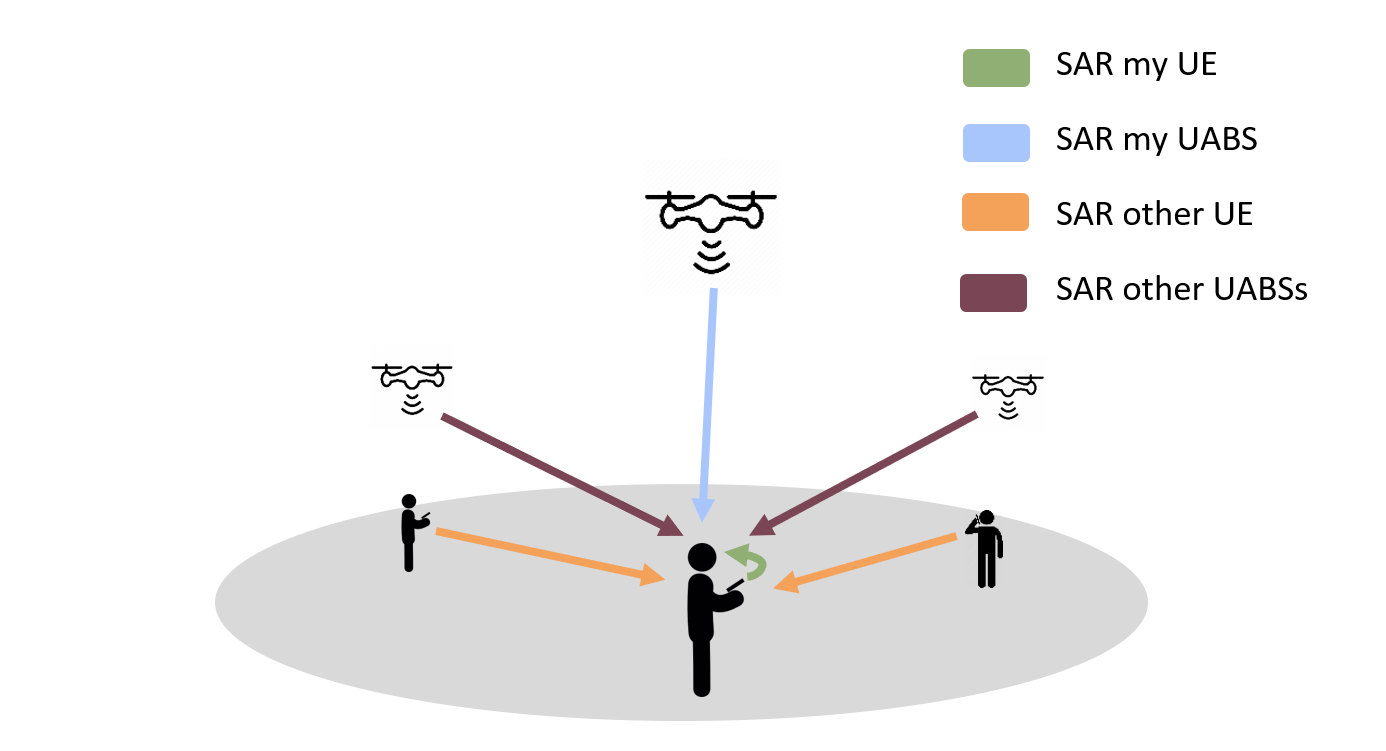
\includegraphics[width=\linewidth]{networkIllustrationSARSources.png}
  \caption{Deze illustratie toont hoe de gemiddelde gebruiker (hier getoond in het midden) be\"invloed worden door verschillende bronnen van elektromagnetische straling.}
  \label{fig:networkIllustration}
\end{figure}

\subsubsection{Electromagnetische straling van een indivuele bron}
\label{sec:calculatingexposure}

De elektromagnetische veldsterkte berekenen in een bepaald punt in het verre veld wordt gedaan worden voor alle \gls{UABS}'en en 
alle mobiele apparaten behalve het apparaat in dat punt. Dit zal namelijk straling in het nabije veld zijn en dient anders berekend te worden. 
De elektromagnetische veldsterkte $E$ voor het individu $u$ komende van een brom $i$ wordt als volgt berekend.

\begin{equation}
E_i(u) [V/m] = 10^{\frac{ES(u)[dBm] - 43.15 + 20*\log(f [MHz])- PL(u) [dB]}{20}}
\label{eq:singleexposure}
\end{equation}

Het berekenen van de effectieve straling (ES) voor een gebruiker $u$ vereist eerst om de  \gls{EIRP}-waarde te hebben berekend 
 \cite{J6_originalExposureFormula,J1}. Dit kan bekomen worden door de zendvermogen $P_t$ op te tellen met de zendversterking $G_t$
 en het aftrekken van het kabelverlies $L_t$.
 Deze formule dient echter uitgebreid te worden zodoende dat er rekening gehouden wordt met signaalverzwakking die komt met
 verschillende stralingspatronen. Deze waarde hangt af van de hoek tussen de gebruiken en de richting waarnaar de antenne wijst. 
 De signaalverzwakking bij een \gls{isotropicradiator} is altijd nul ongeacht de hoek.
 Dit leidt tot de volgende formule.

\begin{equation}
\begin{aligned}
RRP [dBm] = P_t [dBm] + G_t [dBi]- L_t [dB]\\
     - attenuation(u) [dB]
\end{aligned}
\label{eq:eirp}
\end{equation}

De gebruikte frequentie $f$ in formule \ref{eq:singleexposure} is uitgedrukt in MHz. Aangezien 
\gls{LTE} gebruikt wordt zal deze waarde 2600 MHz bevatten.

Als laatste dient formule \ref{eq:singleexposure} ook het padverlies $PL$ te kennen.
Een geschikt propagatie model dient gekozen te worden. Hier wordt geopteerd voor het 
Walfish-Ikegami model aangezien deze goed presteerd voor femtocell netwerken in stedelijke gebieden \cite{J2}.

\subsubsection{Samenvoegen van meerdere bronnen}

De totale elektromagnetische straling $E_{tot}$ in een bepaald punt, komende van alle verschillende bronnen kan berekend worden 
m.b.v. formule \ref{eq:totalexposure}. Hierin staat $E_i$ voor de elektromagnetische veldsterkte voor dat punt komende van bron $i$
en $n$ staat voor alle bronnen in het verre veld van een bepaalde categorie wat hier ofwel \gls{UABS}'s of mobiele apparaten van andere personen.
$E_{tot}$ zal berekend worden in elk punt waar er zich een gebruiker bevindt.
\begin{equation}
E_{tot} [V/m] = \sqrt{\sum_{i=1}^{n} (E_i [V/m]) ^2}
\label{eq:totalexposure}
\end{equation}

\subsubsection{Omzetten van elektromagnetische veldsterkrte naar \gls{SAR}}

Formule \ref{eq:overallSARwb}  verwacht dat de \gls{SAR} waarden in functie van het volledige lichaam uitgedrukt zijn.
Om de elektromagnetische veldsterkte te kunnen omzetten daar deze \gls{SAR}-waarden dient er een onderscheid gemaakt te worden 
tussen bronnen in het nabije veld ($SAR^{wb,nf}$) en het verre veld ($SAR^{wb,ff}$).
$SAR^{wb,myUABS}_{10g}$ is een bron waarbij de gebruiker zich in het nabije veld bevindt terwijl 
de gebruiker zich voor alle andere bronnen in het verre veld bevindt.

Het omzetten van deze waarden gebeurd door middel van een conversie constante dewelke gebaseerd is op 
Duke van de Virtual Family. Duke is een 34 jarige man met een gewicht van 72 kg, een hoogte van 1.74 en 
een bmi van 23.1 kg/m \cite{J22_plets2015joint}. 
Onderzoek toont aan dat conversie constante voor WiFi in het verre veld $0.0028 \frac{W/kg}{W/m^2}$ bedraagt
en  0.0070 $\frac{W/kg}{W}$ in het nabije veld \cite{J22_plets2015joint}.
WiFi maakt gebruik van het 2400 MHz spectrum wat heel dichtbij \gls{LTE} valt (2600 MHz). Daarom 
wordt in \cite{J22_plets2015joint} aangenomen dat de conversie  constante ook van toepassing is voor \gls{LTE}.

Het berekenen van \gls{SAR} in het verre veld  word bijgevolg als volgt gedaan.

\begin{equation}
S [W/m^2]= \frac{(E_{tot} [V/m])^2}{337}
\label{eq:flux}
\end{equation}
\begin{equation}
SAR^{wb,ff}_{10g} [W/kg]= S [W/m^2]* 0.0028 \left[\frac{W/kg}{W/m^2}\right]
\label{eq:DLconversion}
\end{equation}

De constante is vergelijking \ref{eq:DLconversion} zet de \gls{power flux density} $S$ om  naar de verwachtte $SAR^{ff,wb}_{10g}$.
Om dit mogelijk te maken moet 
de uitkomst van formule \ref{eq:totalexposure} eerst nog omgezet worden naar \gls{power flux density} met behulp van formule
\ref{eq:flux}.

De \gls{SAR} die veroorzaakt wordt door het mobiel apparaat in het nabije veld kan gevonden worden door 
het zendvermogen $P_{tx}$ van het  apparaat te vermenigvuldigen met de conversie constante voor het nabije veld.
\begin{equation} 
SAR^{wb,nf}_{10g} \left[\frac{W}{kg}\right] = 0.0070 \left[\frac{W/kg}{W}\right] * P_{tx} [W]
\label{eq:ulToSar}
\end{equation}

De energie die door het mobiele aparaat wordt gebruikt kan berekend worden met formule \ref{eq:powerUE} \cite{J22_plets2015joint}.
\begin{equation} 
P_{tx}^{UE} = \big\{P_{max} [dBm] , P_{pusch} [dBm] + \alpha * PL [dB] + 10log(M) + \sigma \big\}
\label{eq:powerUE}
\end{equation}

\subsection{Microstrip Patch Antenne}
Een microstrip patch antenne is gekozen vanwege zijn eenvoudige productieproces maar voornamelijk vanwege het
 lage gewicht en aerodynamica wat heel voordelig is wanneer het aan een drone gekoppeld wordt \cite{J13_microstripadvantages}.

De dimensies van de antenne hangen af van de gebruikte frequentie en de eigenschappen van het di\"electrisch substraat.
De antenne zal opereren met een frequentie $f_0$ van 2.6 GHz. 
Elk substraat heeft een di\"electrische constante $\epsilon_r$ dat de doorlaatbaarheid 
van eht substraat aanduid en hangt af van het gebruikte materiaal.
Substraten met een hoge di\"electrische constante en kleine hoogte zullen de dimensies van de antenne reduceren 
terwijl  een lager di\"electrische constante met een hogere hoogte de performantie van de 
antenne zullen bevorderen \cite{J14_antennadesign,J15_antennadesign}. 
Voor dit onderzoek is glas het gekozen substraat vanwege zijn hogere di\"electrische constante
van $\epsilon_r = 4.4$ ten opzichte van andere materialen zoals Teflon met een di\"electrische constante
van $\epsilon_r = 2.2$ \cite{J14_antennadesign}. 
Glass met een hoogte van 2.87 mm 
zal de dimensies van het volledige antenne opperlakte verminderen wat 
voordelig is bij de beperkte ruimte die beschikbaar is op een drone.

\begin{table}[h!]
\centering
\begin{tabular}{|l|c|l|}
\hline
 beschrijving            & symbool          & waarde         \\    \hline
 middenfrequentie      & $f_0$           & 2600 Hz       \\ 
 di\"electrische constante    & $\epsilon_r$    & 4.4         \\ 
 Hoogte van het substraat & $h$             & 0.00287 m    \\ \hline
\end{tabular}
\caption{Overzicht van de configuratie parameters}
\label{table:antennaparas}
\end{table}

De dimensies van de stralingsplaat kunnen berekend worden met de formules uit \cite{J14_antennadesign,J15_antennadesign}.
Dit leidt tot een stralingsplaat van 35.09 mm bij 26.55 mm en  een grondplaat van minstens 52.40 mm bij 43.80 mm.
De resulterende microstrip patch antenne is ge\"illustreerd in figuur \ref{fig:basicpatchantenna} en zal resulteren 
in het stralingspatroon getekend in figuur \ref{fig:radpattern}.
\begin{figure}[h!]
\centering
  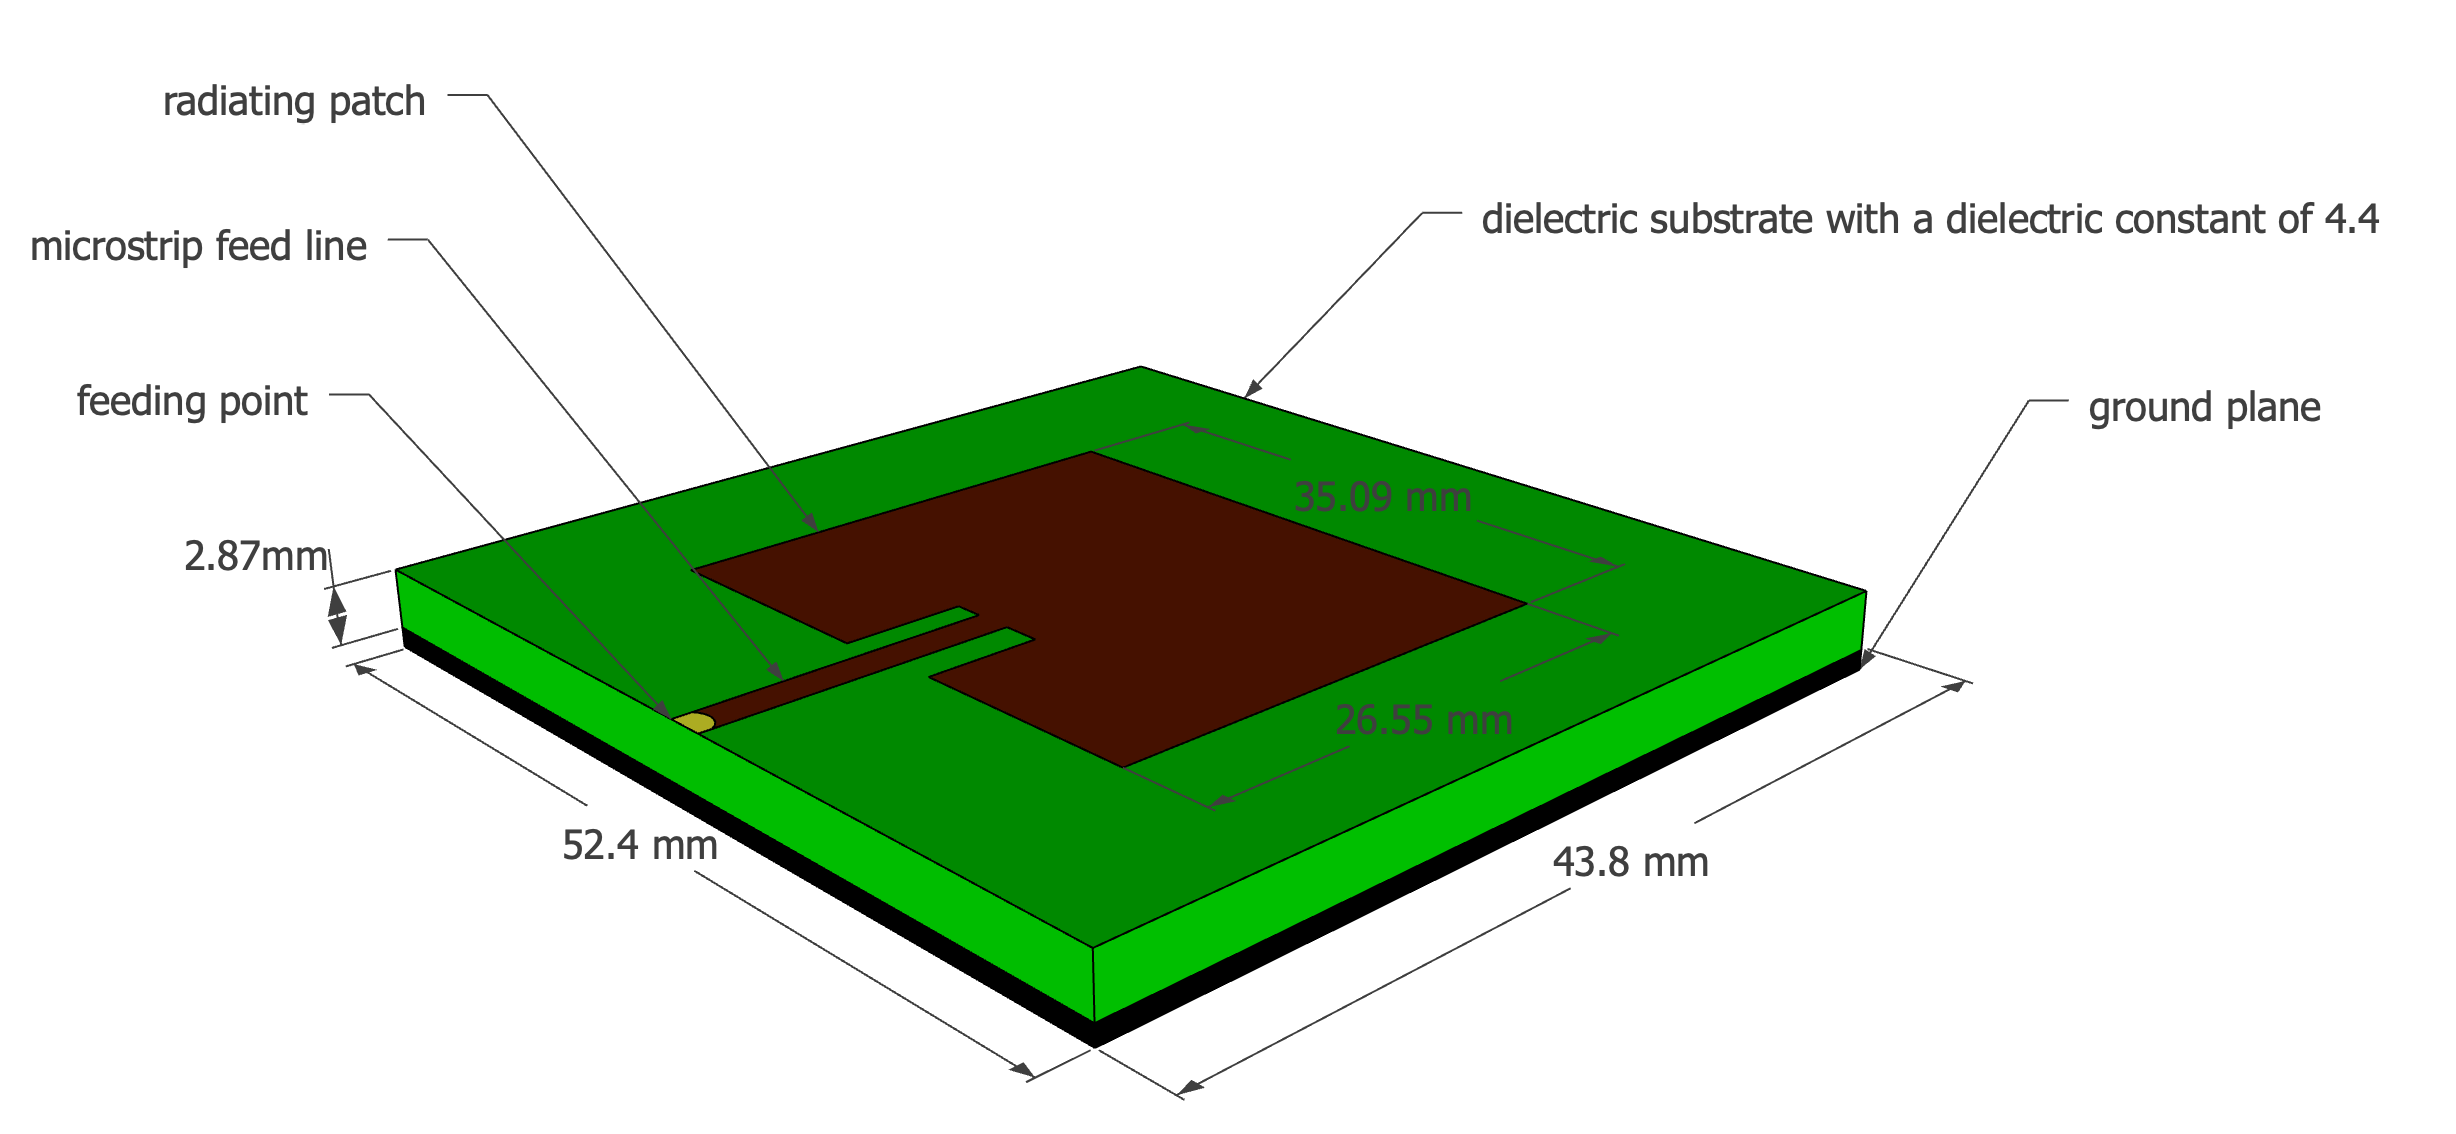
\includegraphics[width=\linewidth]{MicrostripAntenna.png}
  \caption{Design van een microstrip patch antenne.}
  \label{fig:basicpatchantenna}
\end{figure}


\begin{figure}[!htb]
\minipage{0.50\linewidth}
  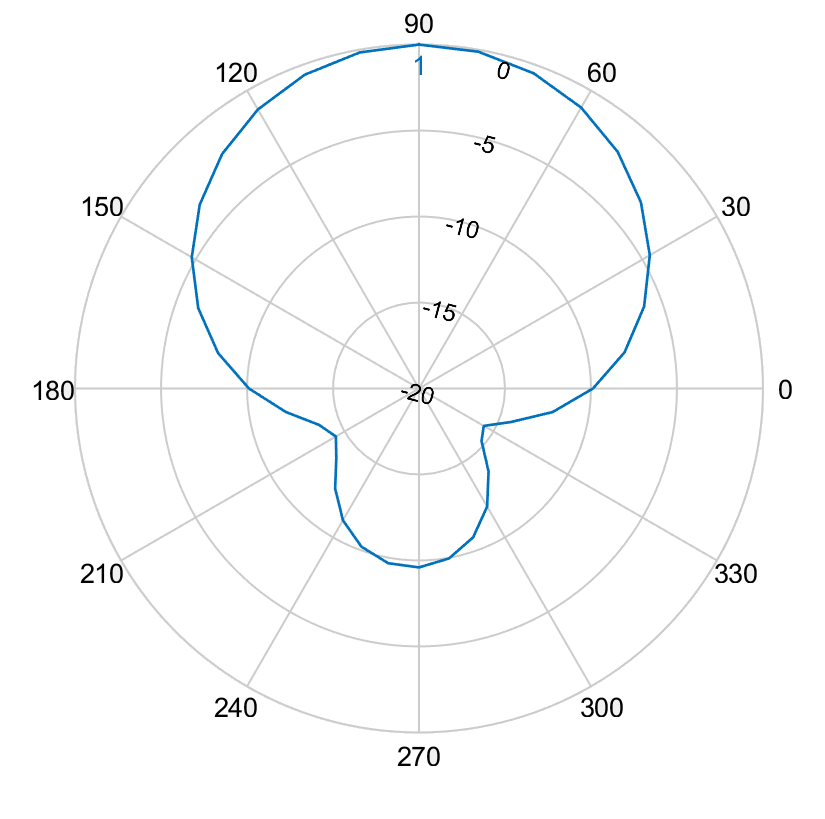
\includegraphics[width=\linewidth]{pattern2/ep.png} 
\endminipage\hfill
\minipage{0.50\linewidth}%
  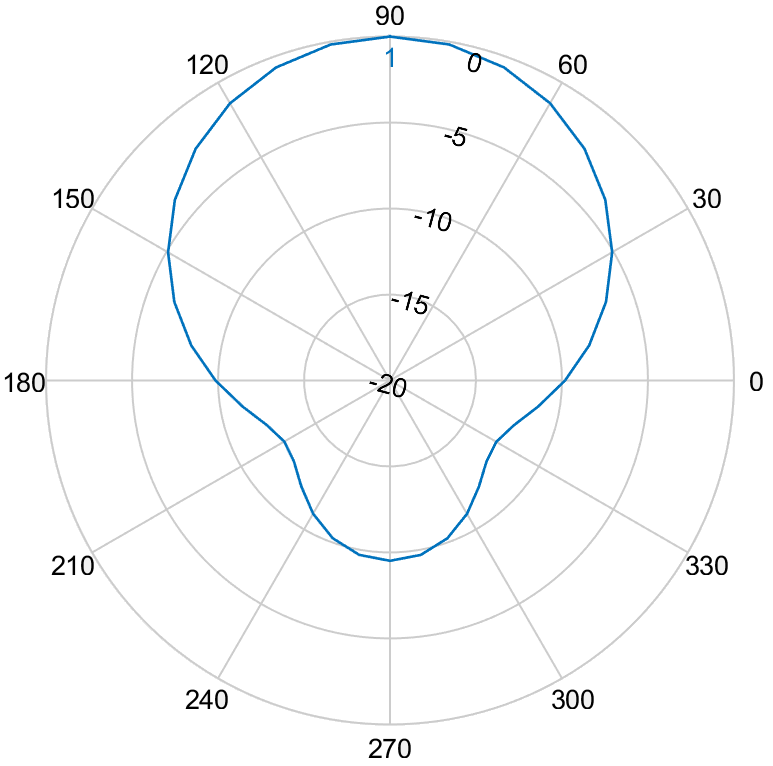
\includegraphics[width=\linewidth]{pattern2/hp.png}
\endminipage
  \caption{Links is het stralingspatroon voor het E-vlak en rechts voor het H-vlak.}
\label{fig:radpattern}
\end{figure}

\subsection{Optimaliseren van het netwerk}

Deruyck et al. bespreekt in \cite{J1} hoe een traditioneel mobiel netwerk geoptimaliseerd kan worden naar
Hoewel een toenemend zendvermogen wel degelijk resulteert in een toenemend elektromagnetische veldsterkte is deze regel niet van 
toepassing indien we het energieverbruik bekijken over het hele netwerk heen. 
De auteurs van \cite{J1} tonen een omgekeerd equivalente relatie aan.
De reden hierachter is dat het vaak goedkoper is op gebied van energie om de elektromagnetische straling van een al actieve base station 
verder te laten toenemen i.p.v.  een nieuwe base station te activeren. Dit leidt tot de volgende fitness functie dewelke
gebaseerd is op \cite{J1}.

\begin{equation} 
f = w * \left(1 - \frac{E_m}{E_{max}}\right) + (1 - w)*\left(1 - \frac{P}{P_{max}}\right) * 100
\label{eq:fitnessfunction}
\end{equation}

Formule \ref{eq:fitnessfunction} geeft een gewicht terug dat aanduid hoe goed het netwerk preseteerd.
$w$ is de belangrijkheidsfactor die loopt van 0 tot 1, grenzen inbegrepen. Een $w$ gelijk aan 0 betekend
dat elektromagnetische straling niet belangrijk is. Een dergelijk network wordt een \gls{PwrC Opt} netwerk genoemd.
Aan de andere kant, een $w$ gelijk aan 1 impliceert dat het minimaliseren van elektromagnetische bloodstelling top prioriteit is
en zal bijgevolg resulteren in een \gls{Exp Opt} netwerk. $P_{max}$ is het energieverbruik van alle \gls{UABS}'s op maximaal 
zendvermogen, ongeacht of ze 
op non-actief staan of niet.
$P$ representeerd de effectieve verbruikte energie van het huidig ontwikkelde netwerk.
$E_m$ is de gewogen elektromagnetische straling van de gemiddelde gebruiken van het huidig ontwikkelde netwerk en 
$E_{max}$ is dezelfde waarde maar met alle \gls{UABS}'s op maximaal zendvermogen.

Bij het optimaliseren van het netwerk is het niet enkel belangrijk om  de gemiddelde gebruiker te overwegen maar ook het limiteren 
van extrema \cite{J1}. 
Daarom wordt er gebruik gemaakt van het gewogen gemiddelde waarbij niet enkel rekening gehouden wordt met de mediaan maar ook 
met het 95\textsuperscript{ste} percentiel. Dit leidt tot formule \ref{eq:em} waarbij 
  $w_1$ en  $w_2$ de gewichten zijn van respectievelijk de mediaan en 95\textsuperscript{ste} percentiel.
 Aangezien verondersteld wordt dat beiden waarden een gelijkwaardige rol spelen zullen beiden een gewicht van 0.5 krijgen. 

\begin{equation} 
E_m = \frac{w_1 * E_{50} + w_2 * E_{95}}{w_1 + w_2}
\label{eq:em}
\end{equation}

\begin{figure}[h!]
  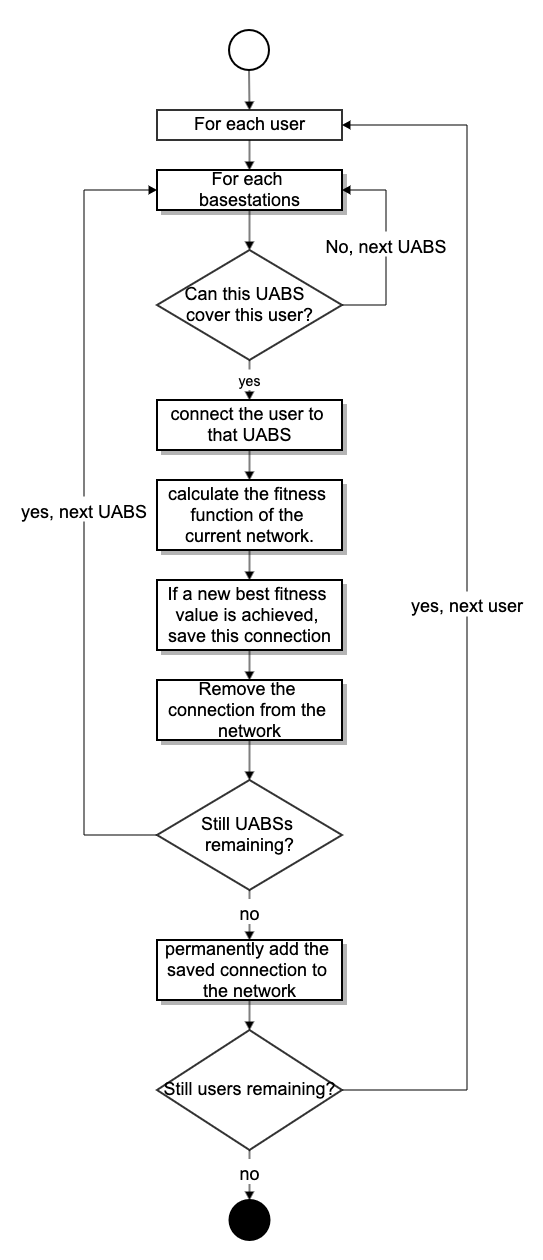
\includegraphics[height=0.8\textheight]{decisionAlgoFlowChart.png}
  \caption{Flowchart of the decision algorithm.}
  \label{fig:decisionAlgoFlowChart}
\end{figure}

\subsection{Simulatie Tool}

\subsubsection{Hoofdalgoritme}
In eerste instantie dient een beschrijving van het gebied voorzien te worden. Dit wordt verwezenlijkt met behulp van 
zogenaamde shape-bestanden. Deze bestanden bevatten een volledige beschrijving van de vorm van elk gebouw. Vervolgens 
worden gebruikers uniform verdeeld over het gebied en zal er een tijdelijke \gls{UABS} geplaatst worden boven elke gebruiker?
Nu is het aan het beslissingsalgoritme om te bepalen welke \gls{UABS}s effectief zal blijven en hoe hoog het zendvermogen van elke \gls{UABS}
zal zijn. Eens het beslissingsalgoritme voltooid is zal de tool controleren of het nummer van online drones niet meer is dat 
de capaciteit van de stockageruimte toelaat. Indien dit wel het geval is zullen drones offline gehaald worden, beginnend bij 
drones die het minste personen behandelen.

\subsubsection{Beslissingsalgoritme}

Het oplossen van het netwerk wordt gedaan door het beslissingsalgoritme en start met het berekenen van het padverlies tussen 
alle gebruikers en tussen gebruikers en drones. Hierna doorloopt het algoritme elke gebruiker waarbij getracht wordt deze te verbinden 
met elke mogelijke drone. Deze verbinding is niet altijd mogelijk omdat een drone al reeds verzadigd kan zijn met andere gebruikers of 
de drone is zo ver verwijderd van deze gebruiker dat het de maximale toegestane zendvermogen zou overschreiden.
Indien een verbinding toch mogelijk is zal de gebruiker met deze drone verbonden worden en zal een score toegekend worden met behulp van 
de fitness functie  \ref{eq:fitnessfunction}. 
Dit proces wordt herhaald voor elke drone. Uitsluitend de verbinding dat resulteert in de beste score voor het volledige netwerk 
zal gebruikt worden. Wanneer de laatste gebruiker behandeld is geweest, bekomen we een volledig netwerk voor een ongelimiteerd aantal drones.
Het network wordt vervolgens terug aan het hoofdalgoritme gegeven voor eventueel verdere afhandeling.
Een stroomdiagram van dit algoritme is gegeven in figuur \ref{fig:decisionAlgoFlowChart}.

%%%%%%%%%%%%%%%%%%%%%%%%%%%%%%%%%%%%%%%%%%%%%%%%%%%%%%%%%%%%%%%%%%%%%%%%%%%%%%%%%%%%%%%%%%%%%%%%%%%%%%%%%%%%%%%%%%%

\section{Scenario's}

De standaard configuratie is gegeven in tabel \ref{table:defaultconf} en is altijd van toepassing tenzij anders vermeld.
\begin{table}[!htb]
\centering
\begin{tabular}[t]{ll}
        \toprule
        \multicolumn{2}{l}{\textbf{Mobiel netwerk}} \\
        \hline
        \hspace{3mm}  technologie        & LTE     \\
        \hspace{3mm}  frequentie         & 2.6 GHz \\
        \hline
        \multicolumn{2}{l}{\textbf{UAV}} \\
        \hline  
        \hspace{3mm}  energie drone        & 13.0 A   \\
        \hspace{3mm}  gemiddelde snelheid        & 12.0 m/s \\
        \hspace{3mm}  gemiddeld energieverbruik      & 17.33 Ah    \\
        \hspace{3mm}  voltage batterij       & 22.2 V \\
        \hline
        \multicolumn{2}{l}{\textbf{Femtocell antenna}} \\
        \hline  
        \hspace{3mm}  maximum $P_{tx}$          & 33 dBm   \\
        \hspace{3mm}  richting van de antenne   & neerwaards   \\ 
        \hspace{3mm}                            & (horizontaal: \ang{0}; verticaal: \ang{90})    \\
        \hspace{3mm}  zendversterking                      & 4 dBm   \\ 
        \hspace{3mm}  kabelverlies               & 2 dBm   \\ 
        \hspace{3mm}  implementation loss       & 0 dBm   \\
        \hspace{3mm}  stralingspatroon         & EIRP or\\
         \hspace{3mm}                           & microstrip patch\\
        \hspace{3mm}  vlieghoogte                & 100m  \\
        \hline
        \multicolumn{2}{l}{\textbf{UE Antenna}} \\
        \hline 
        \hspace{3mm} hoogte                     & 1.5m vanaf de vloer      \\ 
        \hspace{3mm} zendversterking                      & 0 dBm   \\ 
        \hspace{3mm} kabelverlies              & 0 dBm   \\ 
        \hspace{3mm} stralingspatroon         & EIRP  \\
        \hspace{3mm} aantal aanwezig in het netwerk         & 224  \\
        \toprule
\end{tabular}
\caption{Overzicht van de waarden voor een standaard configuratie.}
\label{table:defaultconf}
\end{table}

Drie scenario's zullen onderzocht worden. Het eerste zal \'e\'en enkele gebruiker en drone overwegen 
voor het gehele netwerk. \gls{SAR}, elektromagnetische straling, energieverbruik  en 
het nodige zendvermogen van de antenne zullen onderzocht worden voor verschillende vlieghoogtes.



In a second scenario, the network is expanded for multiple users while still considering only one \gls{UABS}. 
The scenario is divided into two cases. One with a variable flying height but with a fixed 
number of 224 users as is average on an usual day at 5 p.m. in Ghent \cite{J2}.
 In the other case, the number of users varies but the flying height is set to 100 metres \cite{J2}.
The power consumption, electromagnetic exposure and specific 
absorption rate are investigated for each case.

The third scenario is quite similar to the previous scenario. The same two cases are investigated, but now an unlimited number of \gls{UABS}s is avalaible.

Each case from each scenario consists out of four possible configurations.
There are two possible antennae, namely EIRP 
and microstrip patch antenna, which can both be applied in a \gls{PwrC Opt} network or an \gls{Exp Opt} network.

It is important to note that 
all measured values are strictly limited to the sources mentioned in the previous section and thus only cover data traffic 
between \gls{UE} and \gls{UABS}s. Any other potential sources like backhaul links will not be covered.

An overview of the simulation configuration scenarios is presented in figure \ref{fig:fourCasesMatrix}

\begin{figure}[h!]
  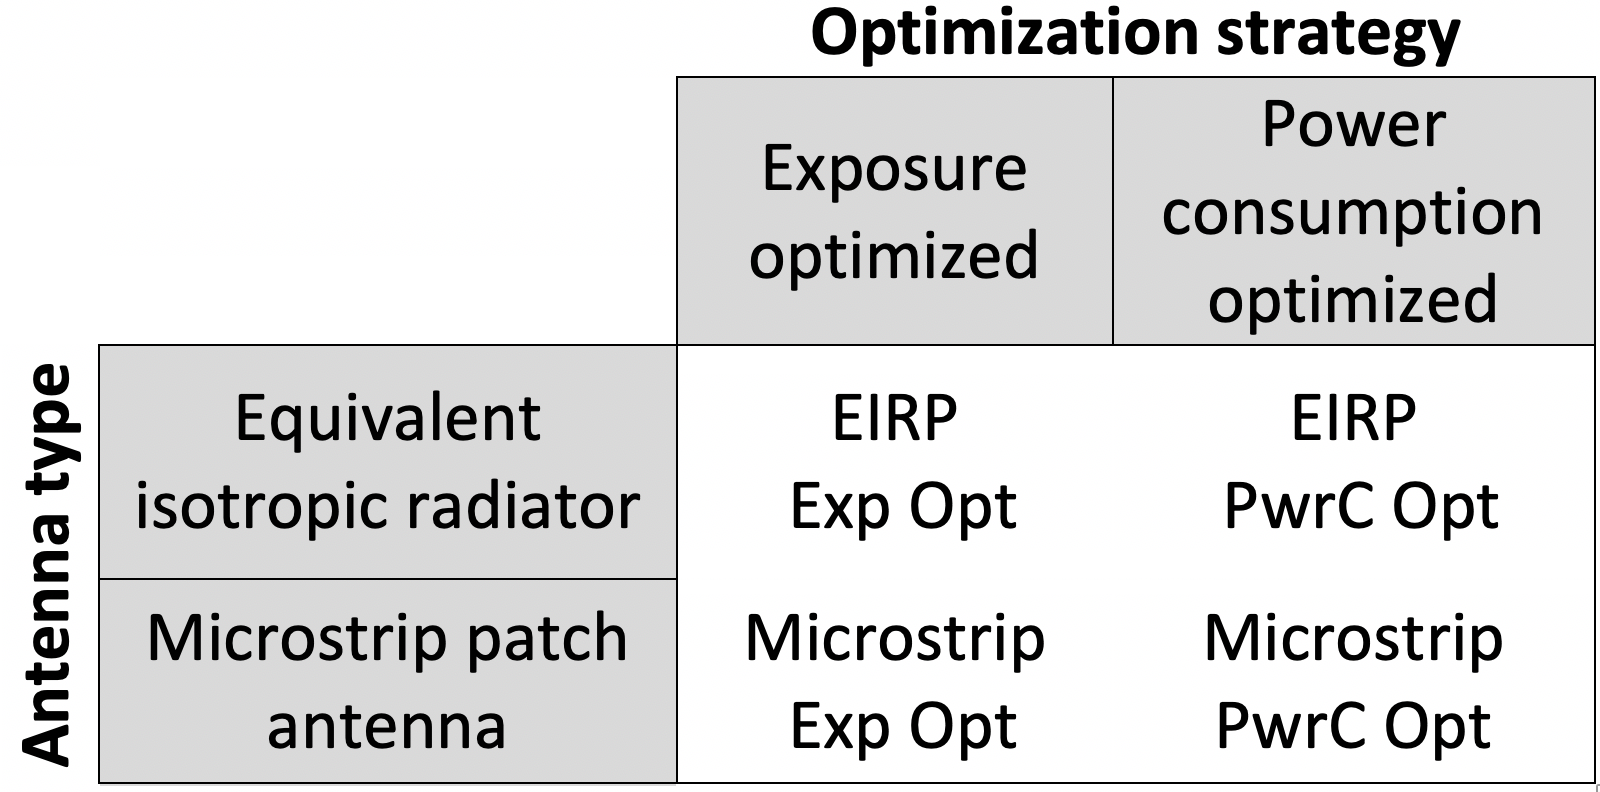
\includegraphics[width=\linewidth]{fourCasesMatrix.png}
  \caption{Matrix with the four possible configurations}
  \label{fig:fourCasesMatrix}
\end{figure}

\section{Results}
\subsection{One User and One \gls{UAV}}

The  results show that for a varying flying height, a logarithmic relationship exists between the $P_{tx}$ and the flying height. 
This is mainly caused by the logarithmic 
scale in which the decibels of the $P_{tx}$ are expressed. So while 10 dBm equals 10 mW, 20 dBm equals 100 mW. 
Each time the flying height becomes too large to cover, the 
$P_{tx}$ increases with one dBm. 
When using the default configuration, with a maximum $P_{tx}$ of 33 dBm,
a \gls{UABS} can fly up to 387 m before losing connection in a free \gls{LOS} scenario.

This scenario is investigated with a microstrip patch antenna using power consumption optimization. 
 However, the chosen optimization strategy does not really matter because the decision 
 algorithm decides which user 
needs to be connected to which \gls{UABS}. Since only one \gls{UABS} is available, both optimization strategies will behave identical.
Further, also the used antenna will not make any difference.
The user is namely positioned in the perfect centre of the main beam where there is 
no attenuation experienced for both antennae.

When investigating this scenario at different flying heights, we notice 
that the \gls{UL} radiation 
increases exponentially while 
the \gls{DL} radiation remains constant during the entire time. The reason that the \gls{DL} radiation
remains constant is because of power control which makes sure that no more power is used than strictly necessary. 
So at lower flying altitudes, there is less path loss and the \gls{UABS} 
will therefore reduce the $P_{tx}$. 
We can therefore confirm that the electromagnetic exposure is a constant fraction of power and distance.
The \gls{UL} radiation starts very low but surpasses the \gls{DL} radiation 
around 80 metres.
%\begin{equation}
%\vec{E} (V/m) = \frac{\Delta U (V) }{\Delta x (m)}
%\label{eq:exposureBasicFormula}
%\end{equation}

\subsection{Increased Population with one UABS}
\subsubsection{Variable Flying Height}
A \gls{PwrC Opt} network has higher exposure compared to an \gls{Exp Opt} network; a behaviour that was already proven by \cite{J1}. 
However, for this scenario, a \gls{PwrC Opt} network will also result in a higher power consumption. 
To understand this, the behaviour of the deployment tool needs to be understood first. 
A \gls{PwrC Opt} network will result in a few high powered \gls{UABS}s because increasing the input power of an antenna costs 
less than activating a new  \gls{UAV}. Likewise, an \gls{Exp Opt} network 
generates a lot of low powered \gls{UABS}s because the lower the power of the antenna, the lower the exposure. This has the consequence that the cover radius 
is less and therefore more UAVs, which cost more energy, are required.
When only a limited amount of \gls{UABS}s are available, 
like only one in this scenario, the tool will only keep \gls{UABS}s which cover the most users. 
Therefore, the power consumption in a \gls{PwrC Opt} network is much more higher. 

Further, the results also show that the exposure increases with higher flying altitudes
because there is a lower probability of having \gls{NLOS} links by obstructing buildings. This has as consequence that  
more users become covered. 
The increasing electromagnetic radiation is however not unlimited.
At even higher
flying altitudes, the distance between a given \gls{UABS} and some users further away becomes too large causing the 
coverage to decrease again. When this decrease occurs depends on the configuration. A \gls{PwrC Opt} 
network tends to decline earlier than an \gls{Exp Opt} network.

When replacing the fictional \gls{EIRP} antenna by a microstrip patch antenna, the percentage of covered users drops for both 
optimization strategies. This is because users, who have a higher horizontal distance between themselves and the \gls{UABS}, 
experience a higher attenuation.

The results further show  
that the radiation from the \gls{UABS} is the main factor followed by the near-field radiation from the user's own device.
The far-field radiation from other \gls{UE} barely contributes anything.

\subsubsection{Variable Number of Users}

Also the results from this case show how EIRP antennae designs are able to cover more users than microstrip patch antennae
just like \gls{PwrC Opt} networks will reach more users than \gls{Exp Opt} networks.
The contribution to the total \gls{SAR} from each individual source is identical to the previous scenario. 

There is still only one \gls{UABS} available. When population grows, more users become uncovered and 
therefore the average electromagnetic exposure decreases.
For example, an EIRP \gls{PwrC Opt} network
will have the highest exposure and therefore covers the most users as opposed to a microstrip patch antenna in 
an \gls{Exp Opt} network which will radiate the least and thus has the lowest number of covered users.

While the population grows, more and more users become uncovered causing the average SAR to drop. 
However, this does not conclude that by increasing the population, the SAR of a user who is directly beneath a \gls{UABS} would be less.
To investigate this, a user is positioned in the middle of the city centre of Ghent and a \gls{UAV} is positioned above him. Initially, only 
49 people are active around him. The \gls{SAR} of our central user is monitored while the population around him is growing.
Figure \ref{fig:connectionMap} shows with the black lines which users are connected. The left map is for only 50 users and 
shows that only one user is connected besides our central user. The map on the right considers 600 users and shows much more connected users.
The results show that the \gls{UL} \gls{SAR} of the central user remains constant; a normal behaviour since the flying altitude does not change.
The \gls{SAR} from the \gls{UABS} experiences a slight increase. When the population grows, more users become available 
and some will spawn near the central user. The \gls{UABS} will likely decide to cover these users as well as visible in figure \ref{fig:connectionMap}.
These users might have a slightly 
worse path loss because of obstructing buildings or a somewhat bigger distance. The \gls{UABS} reacts to this by increasing 
its power consumption causing an increase in the \gls{DL} \gls{SAR} for the central user. The results further also show 
that the \gls{SAR} from other \gls{UE} increases when the population increases. But as mentioned  before, it is much less 
compared to the other sources.

\begin{figure}[!htb]
\minipage{0.50\linewidth}
  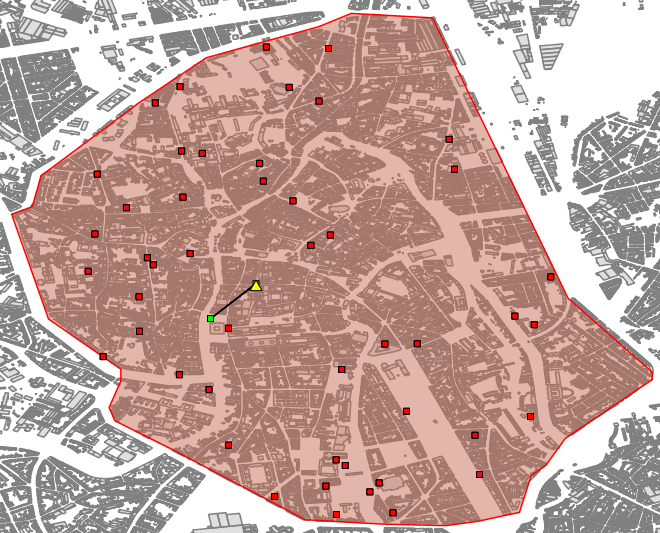
\includegraphics[width=\linewidth]{../images/connectionsMap50Users.png}
\endminipage\hfill
\minipage{0.50\linewidth}%
  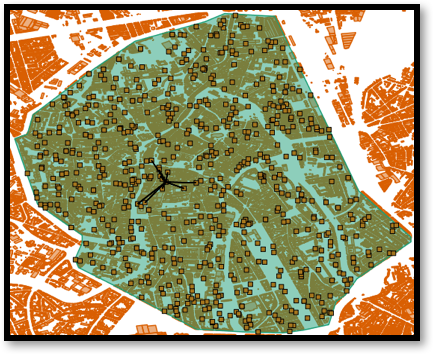
\includegraphics[width=\linewidth]{../images/connectionsMap600Users.png}
\endminipage
  \caption{Overview of which users are connected to the \gls{UABS}. The map on the left is for 50 active users while the map on the right considers 600 active users.}
  \label{fig:connectionMap}
\end{figure}

\subsection{Unlimited Number of UABSs}
\subsubsection{Variable Flying Height}
The same cases as in the previous scenario are investigated. Only now, an unlimited number of \gls{UABS}s is available.
The results prove that the different optimization strategies work as intended.
\gls{PwrC Opt} networks have indeed a lower power consumption but therefore result in higher electromagnetic radiation.
On the other hand, an \gls{Exp Opt} network will reduce the electromagnetic exposure by using more \gls{UAV}s and thence also increase the network's
power consumption.
This conclusion was already made in \cite{J1} and is supported by these results.
\begin{figure}[h!]
  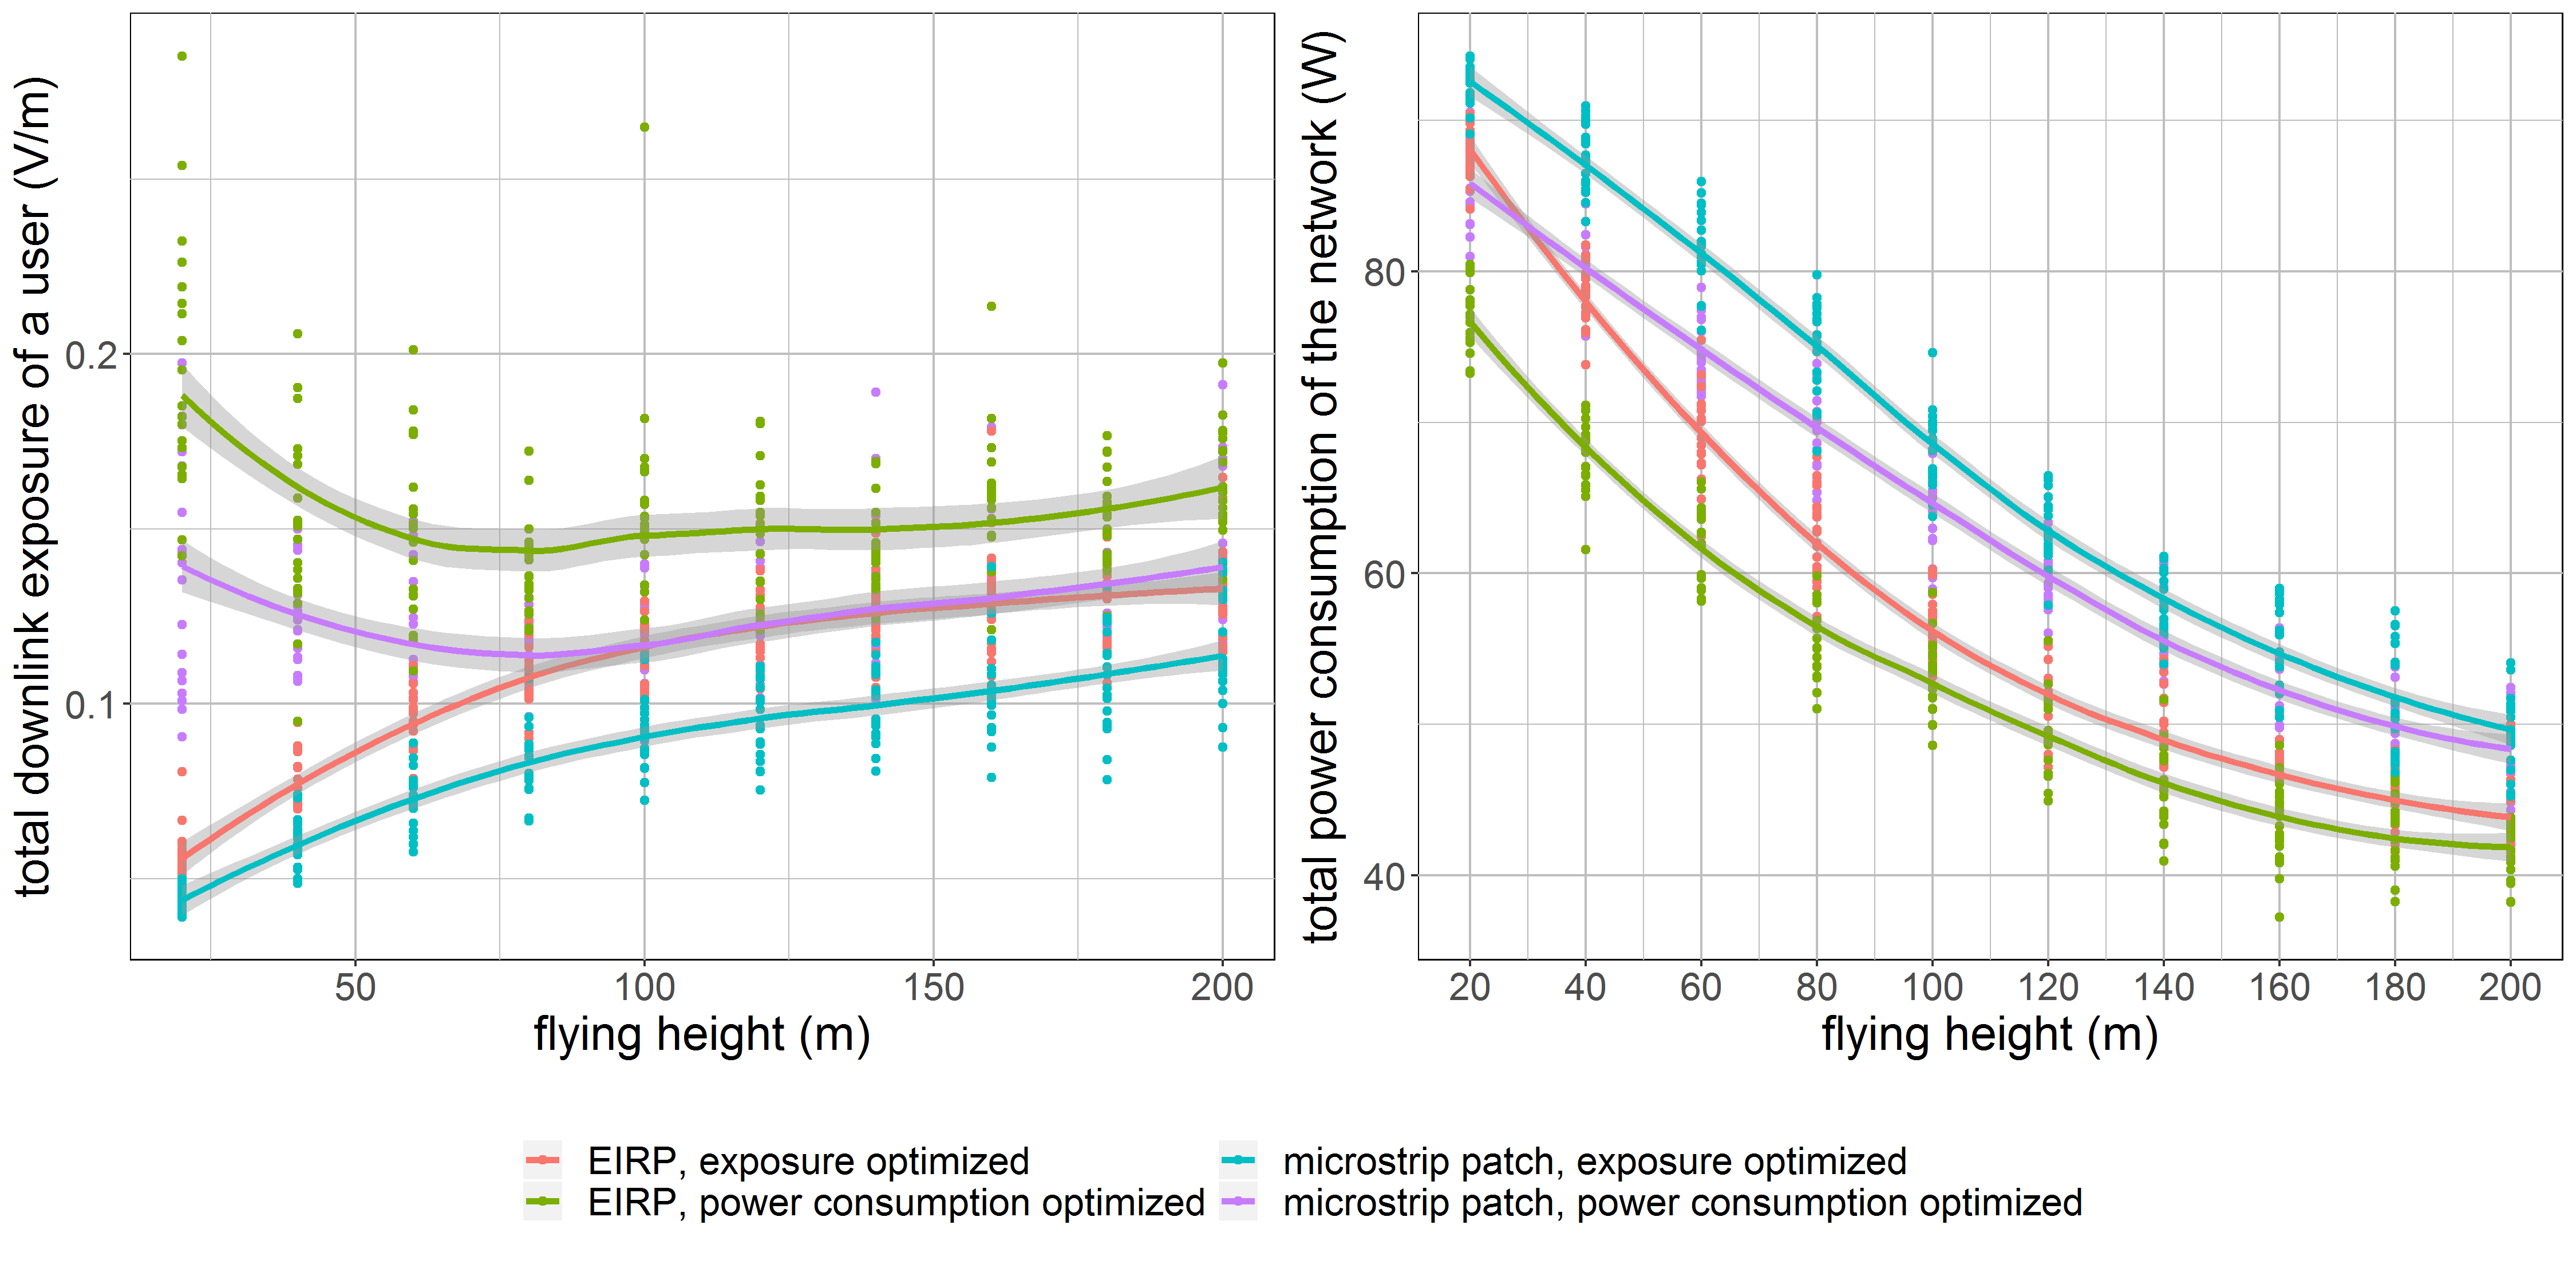
\includegraphics[width=\linewidth]{../results/s3/fhvsdlAndPc.png}
  \caption{These two figures show how the flying height influences the downlink electromagnetic radiation of the average user (left) and 
  power consumption of the entire network (right) for an unlimited number of drones.}
  \label{fig:s3a_dlAndPc}
\end{figure}

The exposure in figure \ref{fig:s3a_dlAndPc} shows that an \gls{Exp Opt} network increases logarithmically while the \gls{PwrC Opt} network rather 
has a concave relationship with the flying height, and has its lowest point at around 70 metres.

At a flying height of 20 m, the \gls{Exp Opt} network has on average 220 to 224 \gls{UABS}s. That is (almost) one \gls{UABS} for each user
so it is logical that the electromagnetic exposure is very low.
The number of \gls{UAV}s in a \gls{PwrC Opt} network is much less in order 
to save energy but it is still able to achieve the same percentage of coverage.
This is done by increasing the radiation so the cover radius would become larger.
The results further show that the network profits from increasing the flying altitude. Not only
less \gls{UAV}s are needed but also the power consumption is lower. Both can be explained by the
lower path loss when UABSs fly higher. 

Figure \ref{fig:s3a_fourSourcesMatrix} shows how each source contributes to the total \gls{SAR}.
A first consequence of higher flying altitudes is the increase in electromagnetic radiation from the user's own device; a behaviour also explained in the first scenario.
A second  consequence is that also 
 the exposure from `other \gls{UABS}s' increases, caused by lower path loss from less obstructing buildings.
The figures from \ref{fig:s3a_fourSourcesMatrix} further also clearly show that this increase 
in electromagnetic radiation will be less for a microstrip patch antenna. The reason behind this is that energy 
will be more focussed towards the ground and there is less sideways radiation because of attenuation.

\begin{figure}[h!]
  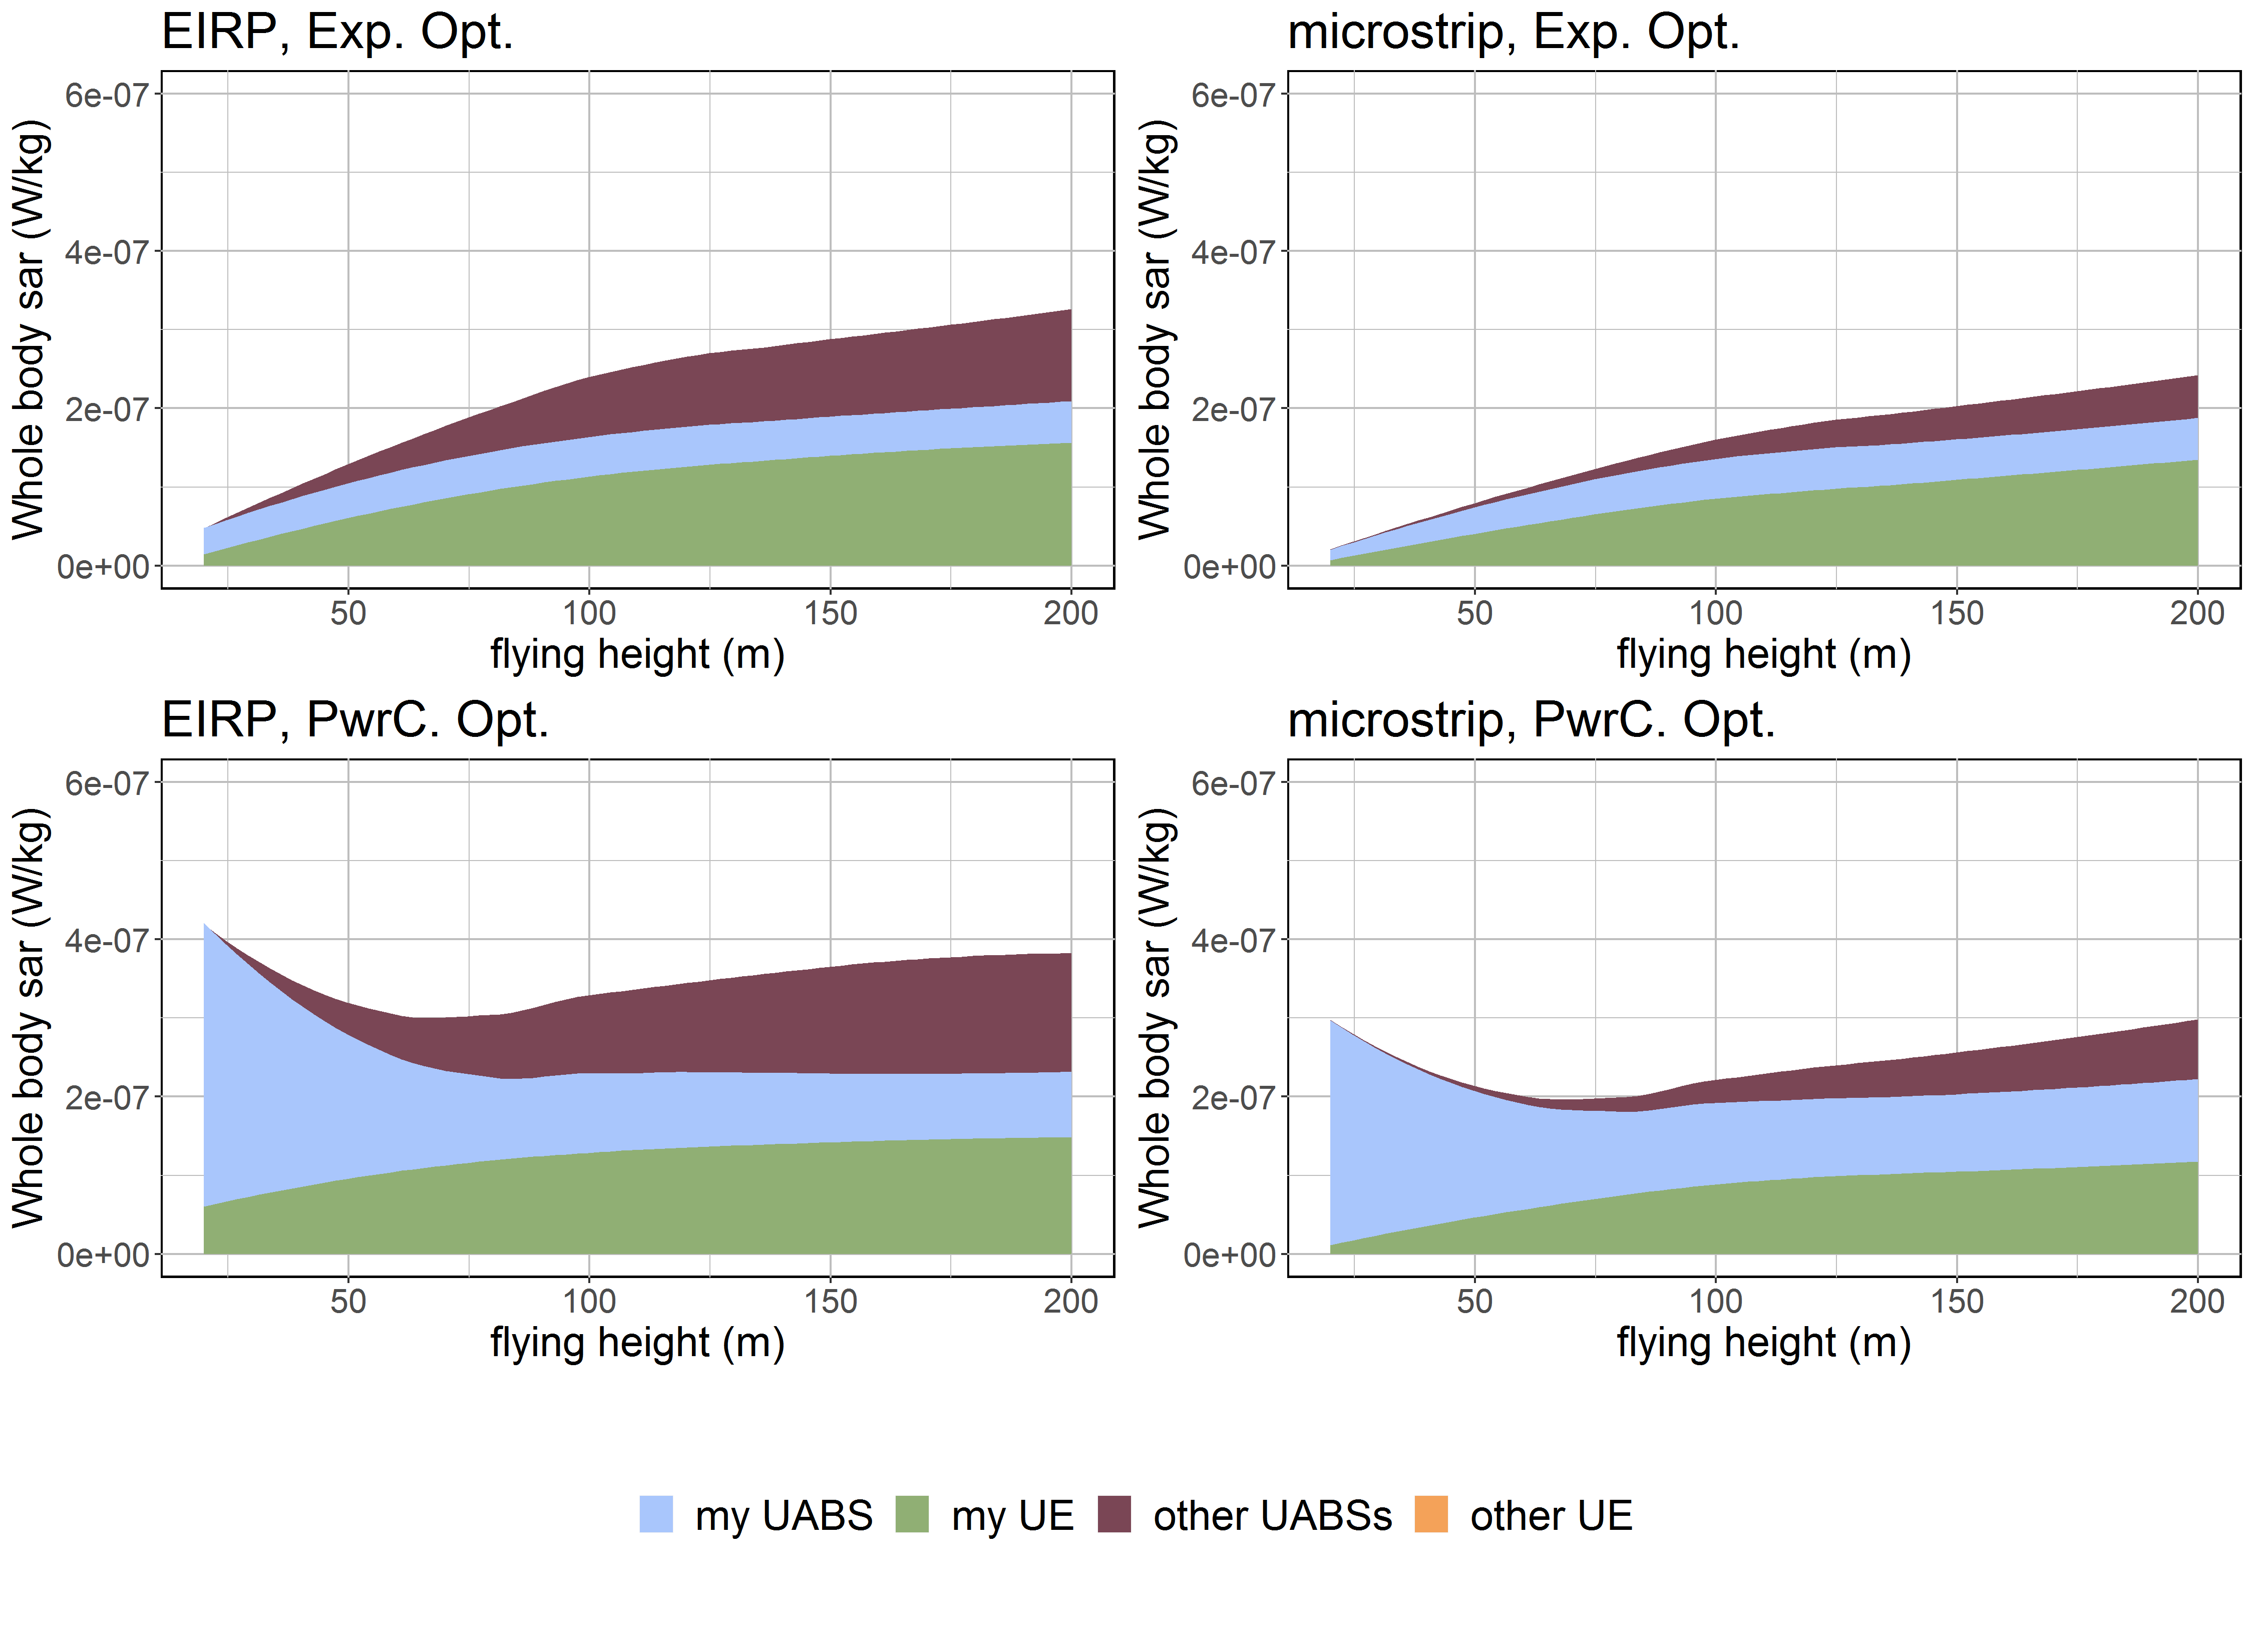
\includegraphics[width=\linewidth]{../results/s3/fhFourSources.png}
  \caption{Each chart corresponds with one of the four possible configurations. The contribution of each source towards the total 
  \gls{SAR} for a varying flying height is shown.}
  \label{fig:s3a_fourSourcesMatrix}
\end{figure}

\subsubsection{Variable Number of Users}
When the flying height of the \gls{UABS}s is fixed to 100 metres and the density of the population increases, also 
the number of required \gls{UAV}s increases in order to reach a 100 \% coverage.
Figure \ref{fig:s3b_dlAndPC} shows that when the number of \gls{UABS}s and users increases, 
also the electromagnetic exposure and power consumption increases.
Once again, the EIRP antenna in a power consumption network has the highest exposure for the lowest power consumption
and a microstrip patch antenna in an \gls{Exp Opt} network the lowest exposure for the highest power consumption.
The two other combinations are in the middle and behave very similar.

\begin{figure}[h!]
  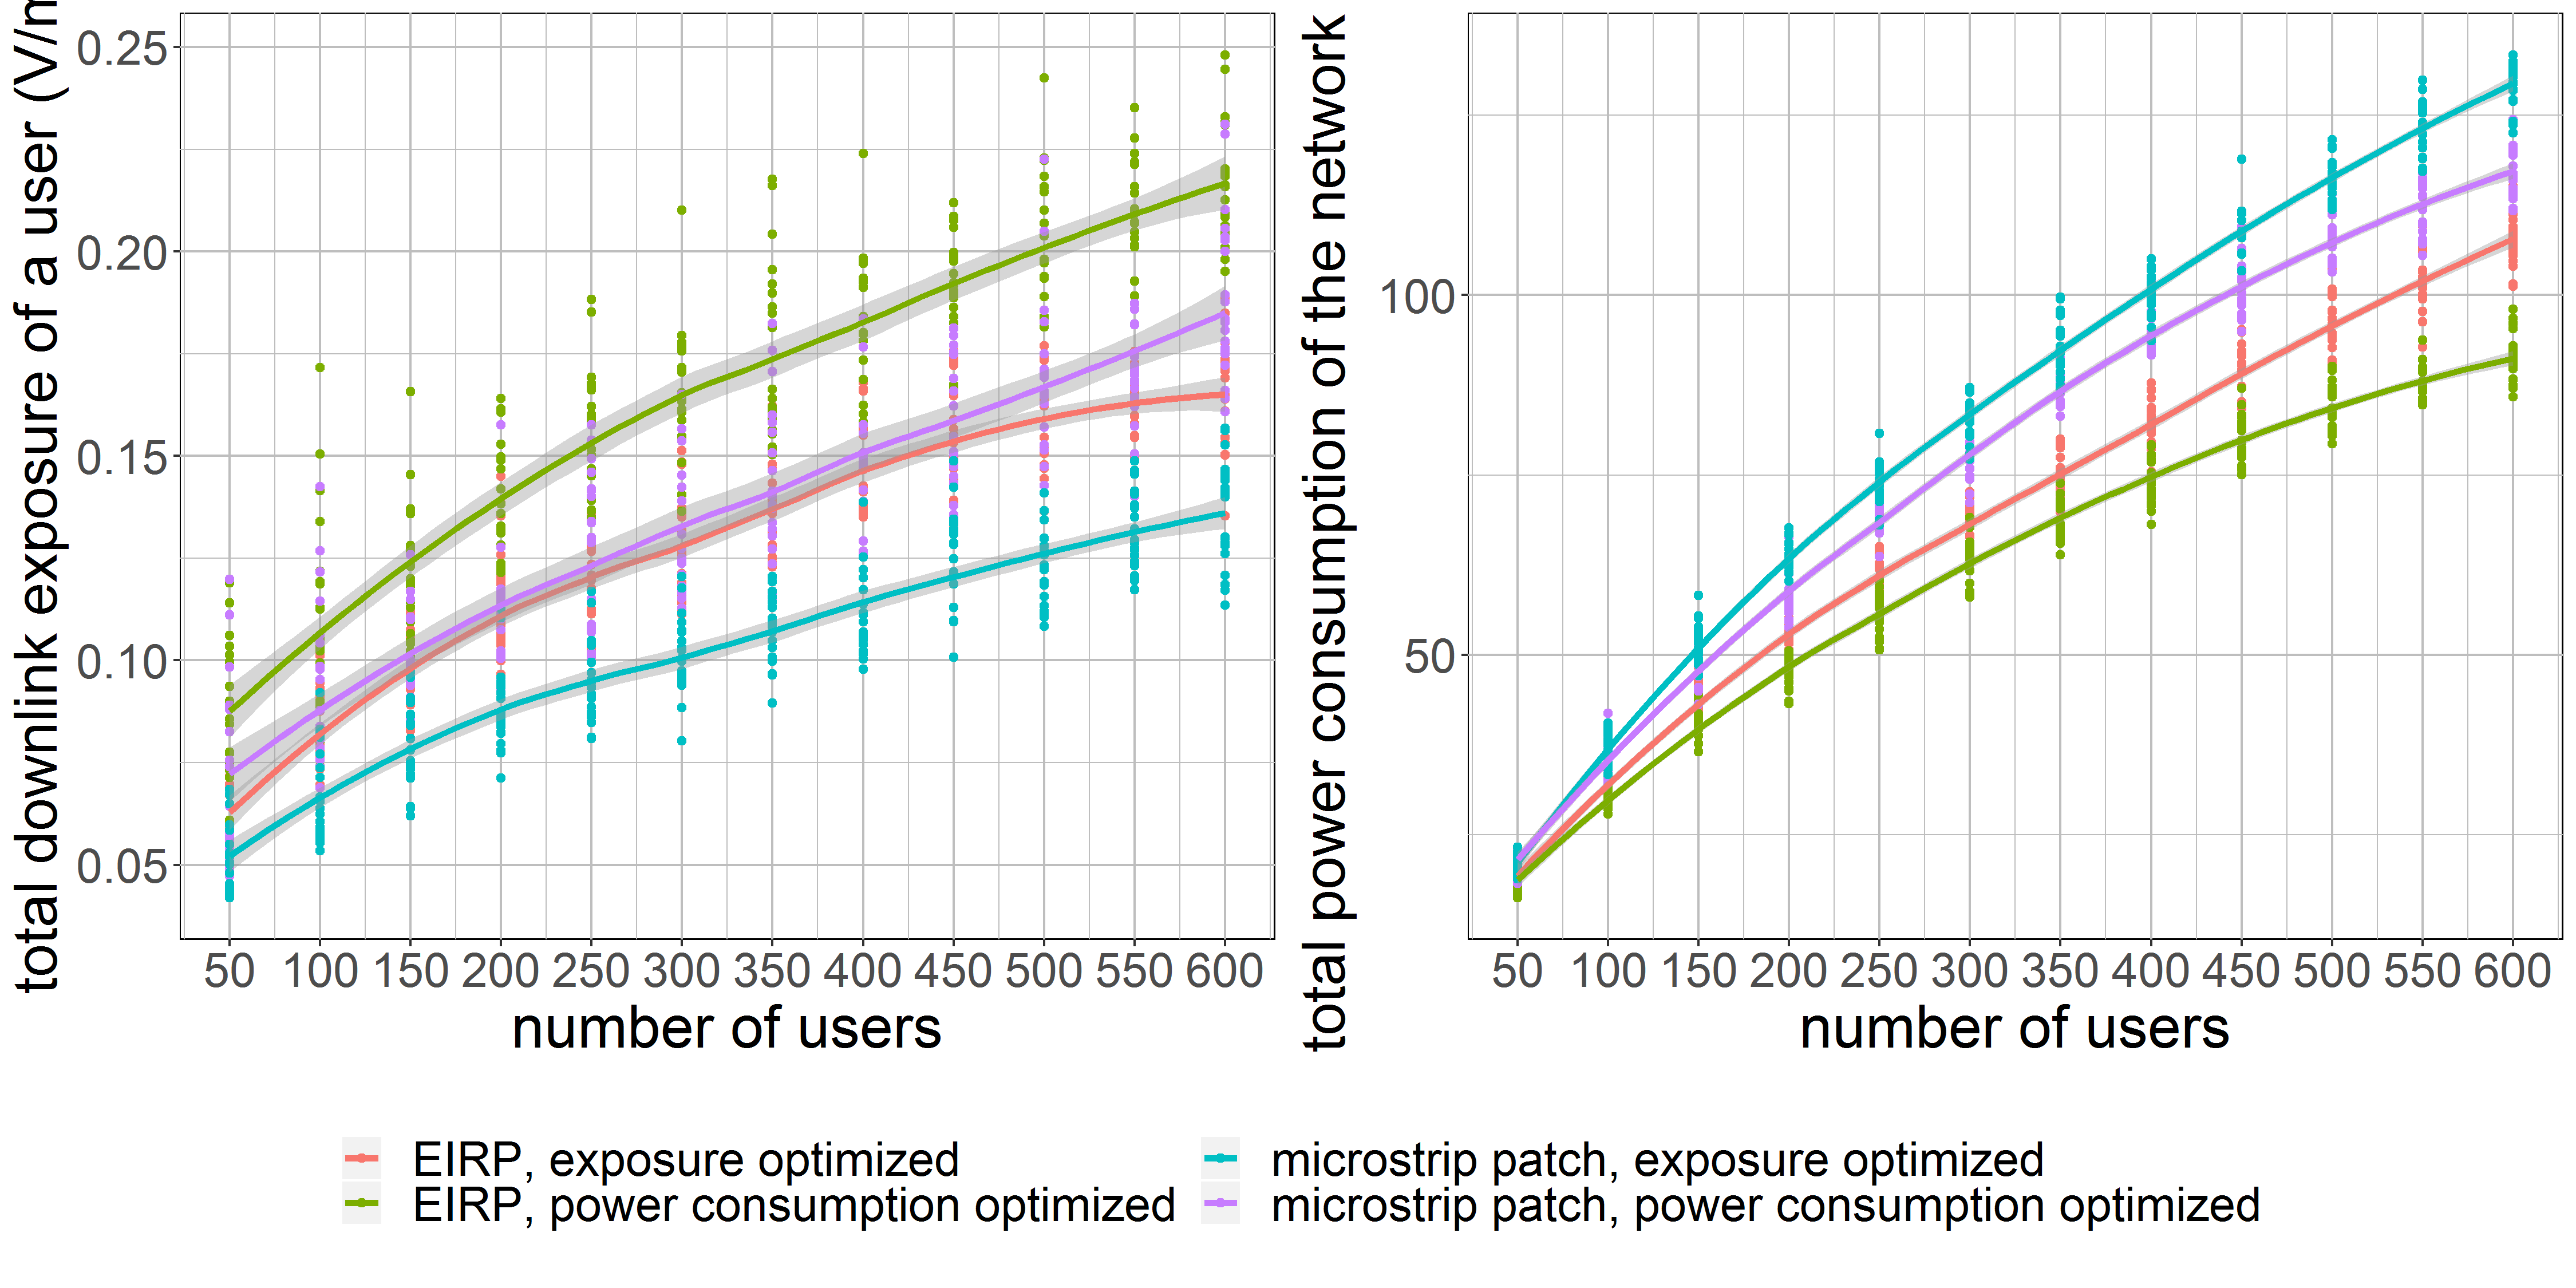
\includegraphics[width=\linewidth]{../results/s3/uvsdlAndPc.png}
  \caption{These two figures show how the number of users influences the downlink electromagnetic radiation of the average user (left) and 
  power consumption of the entire network (right) for an unlimited number of drones.}
  \label{fig:s3b_dlAndPC}
\end{figure}

When looking at the different contributions to the total \gls{SAR} in figure \ref{fig:s3b_fourSourcesMatrix}, 
we see that the weighted average 
\gls{SAR} from the users' own device and from the serving \gls{UABS} remains constant. The flying altitude is always the same so 
also the required energy to cover that distance will remain the same. 
The only \gls{SAR} values that increase are the \gls{DL} \gls{SAR} from other \gls{UABS}s and the \gls{UL} \gls{SAR} 
from other \gls{UE}. 
When more users come online, also more \gls{UAV}s will be radiating. The electromagnetic
radiation will thus increase for both types of sources. Moreover, there is very little path loss at this flying altitude since it 
is higher than the average building.

\begin{figure}[h!]
  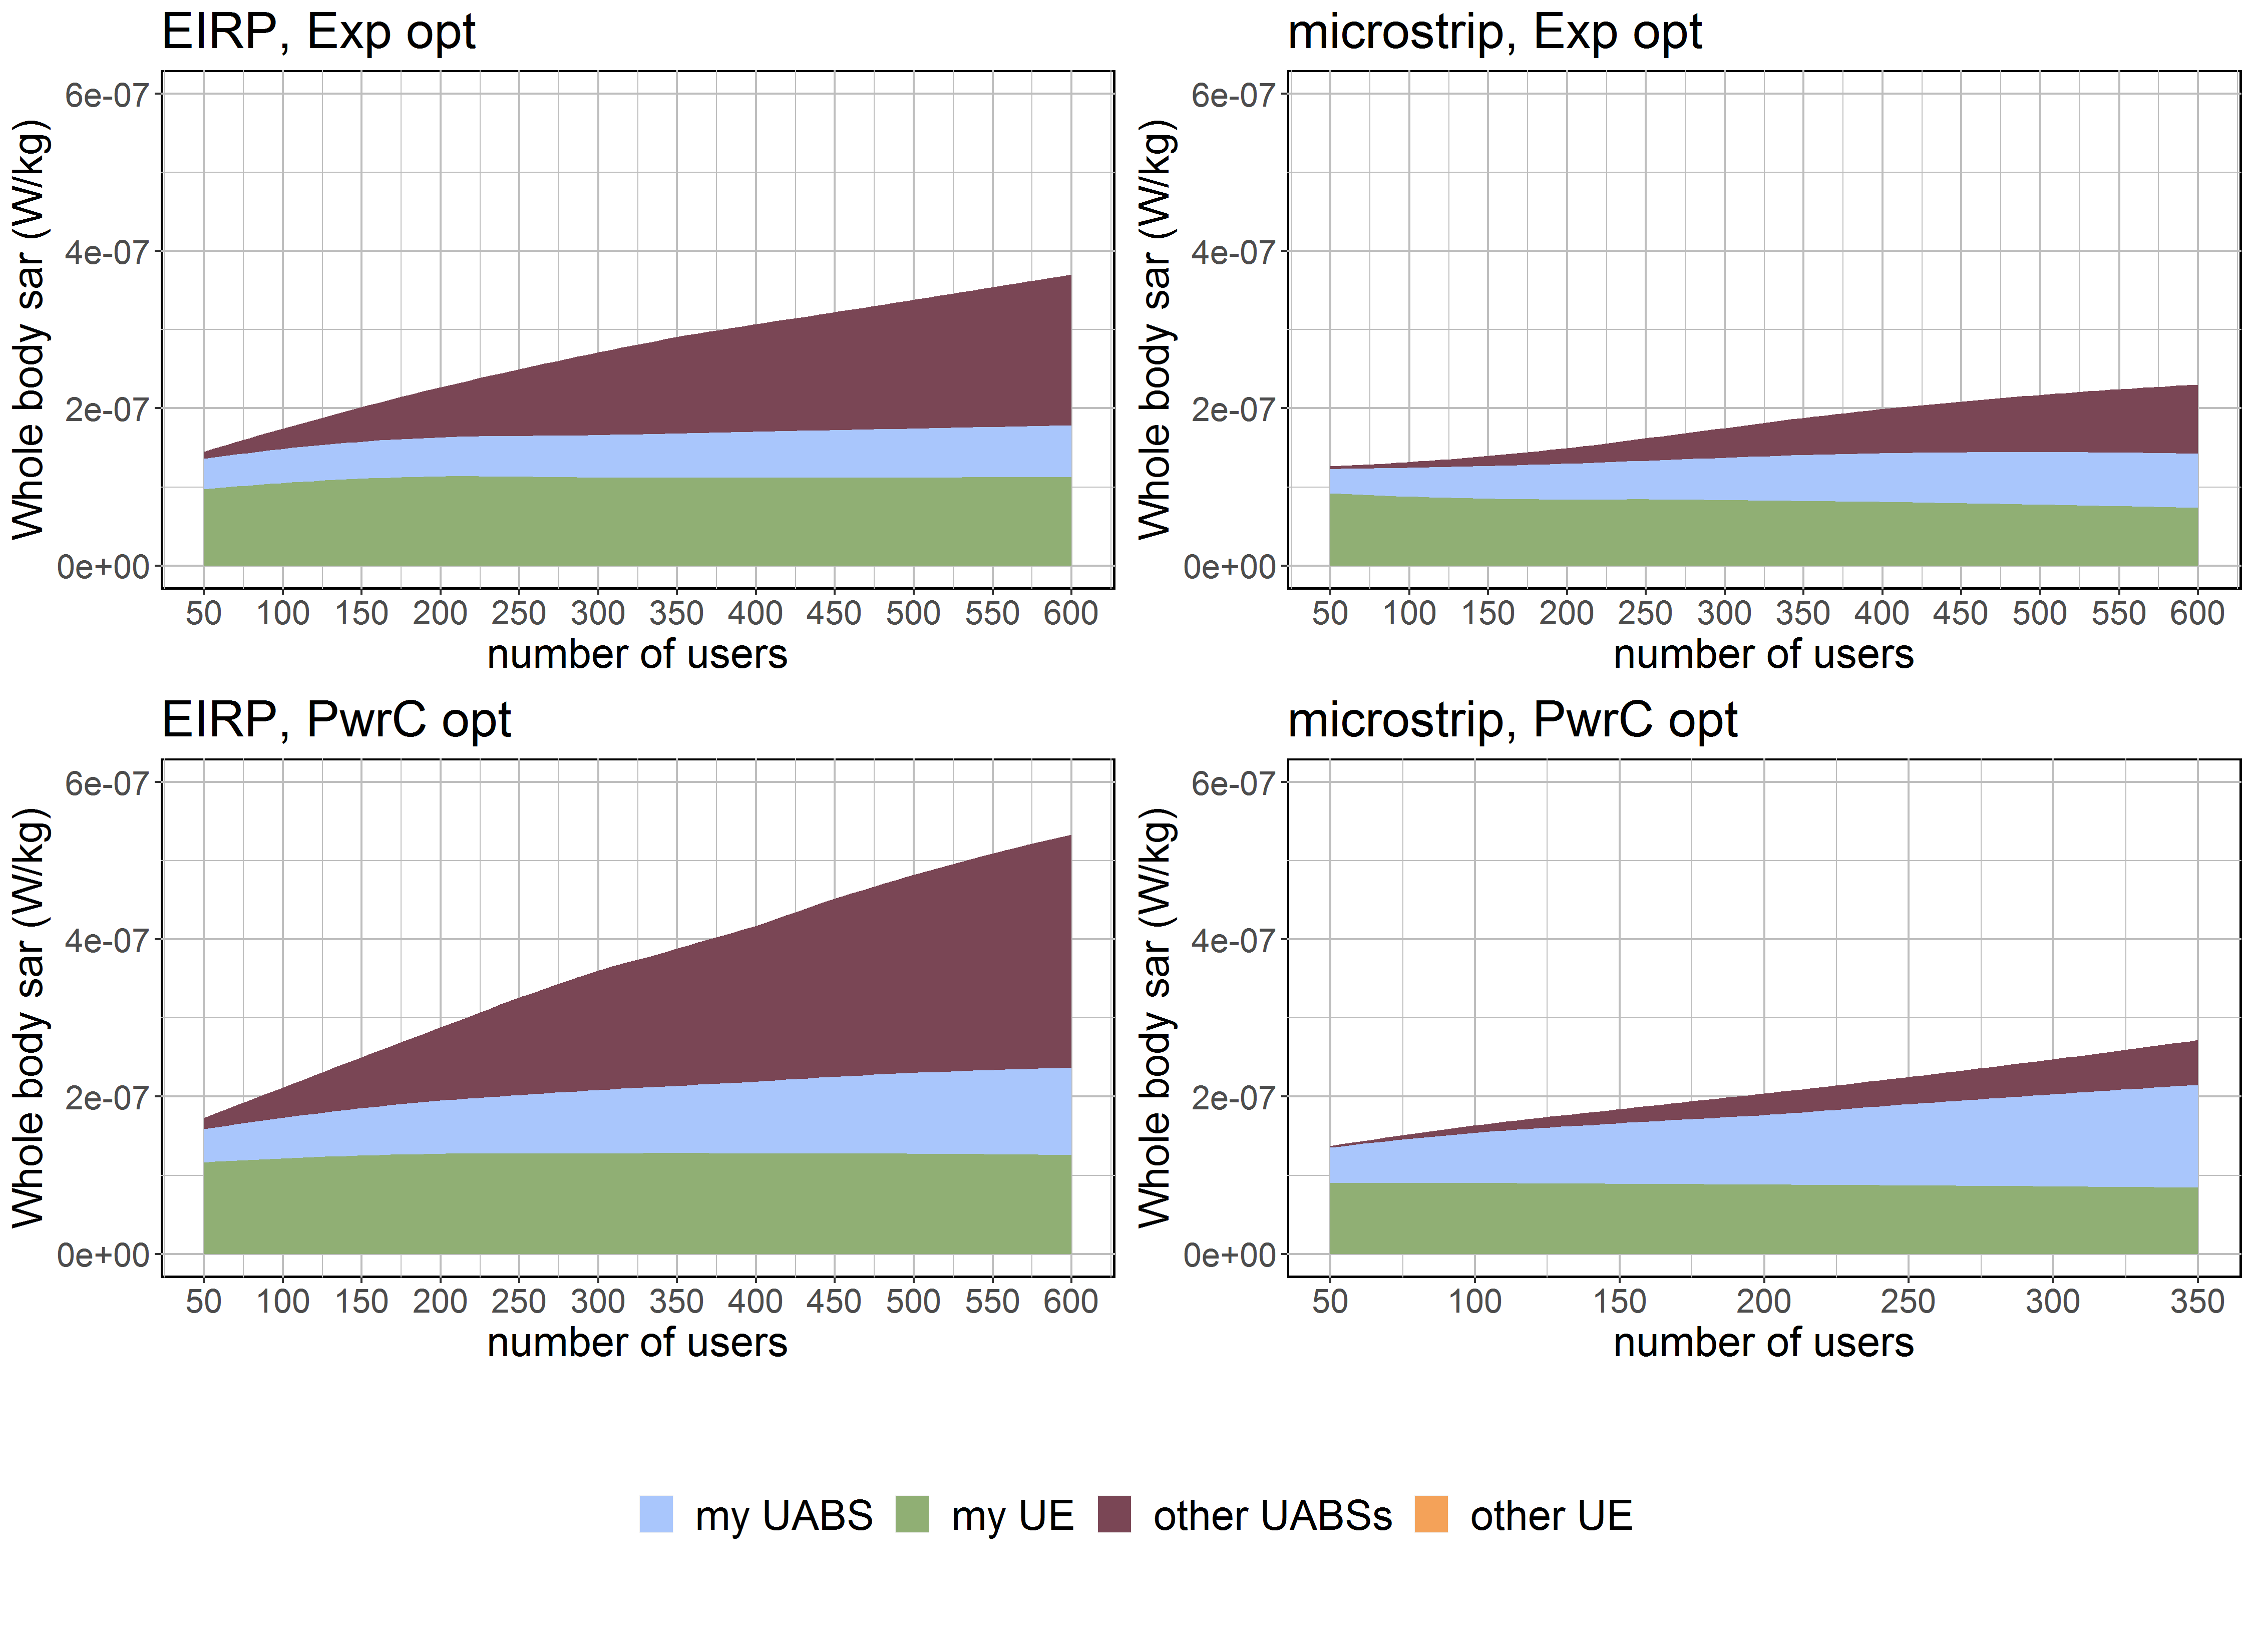
\includegraphics[width=\linewidth]{../results/s3/uFourSources.png}
  \caption{Each chart corresponds with one of the four possible configurations. The contribution of each source towards the total 
  \gls{SAR} for a varying number of users shown.}
  \label{fig:s3b_fourSourcesMatrix}
\end{figure}

\section{Conclusion}
%How can a UABS network be optimized to minimize global exposure or overall power consumption? 
Literature showed that a network can be optimized towards either the power consumption of the entire network 
or the electromagnetic exposure of the average user using a fitness function \cite{J1}.
However, the fitness function should be used with care considering that \gls{UABS}s can be placed anywhere as opposed to 
the transmission towers from \cite{J1} who have a predetermined position. 
In an \gls{Exp Opt} network, this causes a lot of users to get a \gls{UABS} all by 
themselves because this is the best approach to minimize exposure.
A \gls{PwrC Opt} network on the other hand will try to limit the number of drones 
in order to save energy. 
So as a rule of thumb: an \gls{Exp Opt} network will result in a lot of low powered devices (increasing the overall power consumption)
while a \gls{PwrC Opt} network results in a few high powered devices (increasing the exposure of the average user).
If the goal is to remain in the air for a longer period of time, an \gls{Exp Opt} network is recommended because the power consumption of 
an individual \gls{UABS} is lower.
On the other hand, a \gls{PwrC Opt} network is cheaper because less drones are involved. 
Moreover, the results show that the electromagnetic radiation in a \gls{PwrC Opt} network (with high powered \gls{UABS}s)
is far below the thresholds enforced by the Flemish government.

The user's main sources of exposure are the user's own device and the \gls{UABS} who is serving him, followed by all
other \gls{UABS}s in the network. 
When the population increases, there is not only more radiation from \gls{UE} but also 
from more \gls{UABS}s that are serving the other users.
The exposure from other people's \gls{UE} is so low that it can be neglected.
An \gls{Exp Opt} network will limit the total exposure mainly by trying to reduce the exposure from other \gls{UABS}s.

%1)	How does the network behave differently after the introduction of a realistic antenna?
A directional microstrip patch antenna is introduced because it gives several advantages compared to omnidirectional antennae.
Directional antennae are able to focus their energy there where it is needed, namely towards the ground. Microstrip patch antennae 
further benefit from their thin and lightweight design. The performance 
of this directional microstrip patch antenna has been compared to a 
fictional \gls{isotropicradiator}.
This \gls{isotropicradiator} has higher exposure and coverage for less power, compared to realistic antennae like microstrip patch antennae
because of the absence of attenuation, and can hypothetically be compared with an antenna with a very big aperture angle.
This type of antenna can achieve the same coverage with less
resources like power and number of drones. 
A microstrip patch antenna with a more limited aperture angle of \ang{90} requires more resources but 
causes less sideways radiation. So the exposure from other \gls{UABS}s will be way less.

\begin{figure}[h!]
  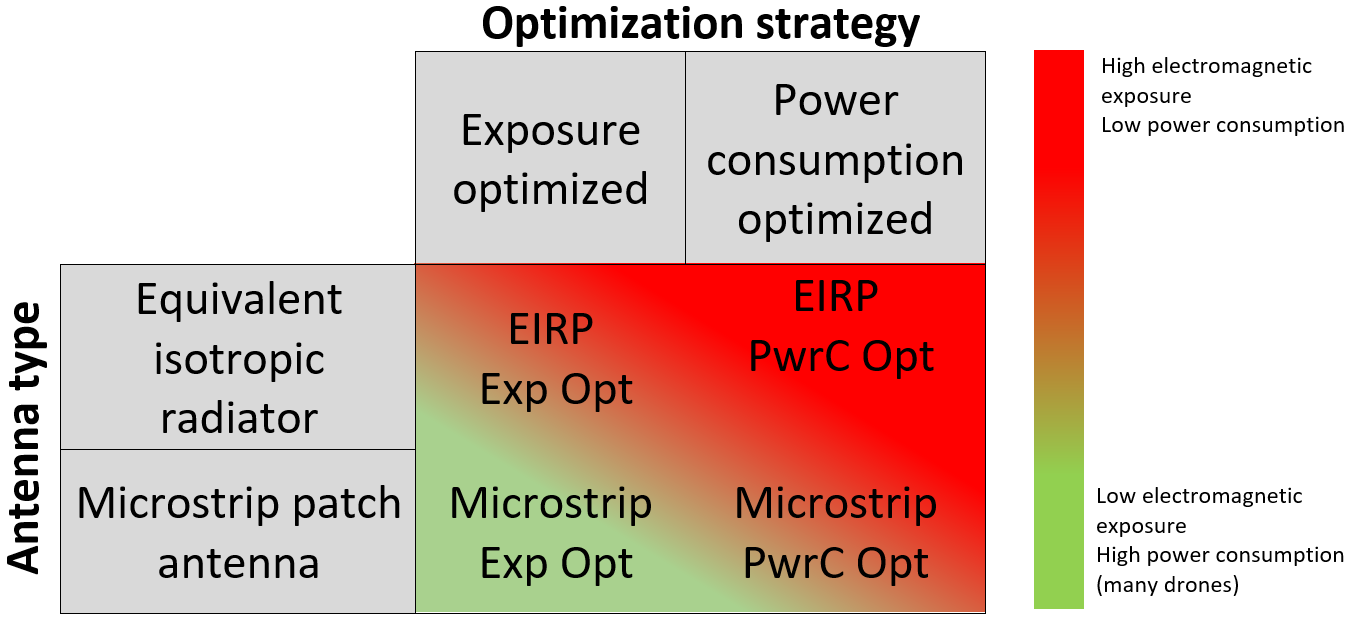
\includegraphics[width=\linewidth]{fourCasesMatrixSol.png}
  \caption{Matrix with the four possible configurations, colour-coded based on the results.}
  \label{fig:resultIllustration}
\end{figure}

Remarkable is that an \gls{EIRP} \gls{Exp Opt} network behaves very similar to a microstrip \gls{PwrC Opt} network as shown 
in figure \ref{fig:resultIllustration}.
This results in the best of both worlds. 
The microstrip patch antenna will generate less electromagnetic radiation by design and
 the power consumption optimization reduces the number of required drones and power. A microstrip patch antenna with an aperture 
 angle of \ang{90} is considered as a good solution but if budget is limited, an antenna with a larger aperture angle 
 would further reduce cost without interfering with the Flemish legislation regarding electromagnetic exposure.

The electromagnetic radiation of an \gls{Exp Opt} network increases with higher flying altitudes.
Around 80 metres, the exposure from the  user's device surpasses the exposure from the serving \gls{UABS}.
On the other hand, a \gls{PwrC Opt} network shows that the lowest exposure is measured around 70 to 80 metres.
Further, the results also show that the number of required drones decreases when the flying height becomes larger; a conclusion that was also made in \cite{J2}.
When also considering the results from \cite{U1} where a flying altitude from 
80 metres is suggested for an optimal access and backhaul connectivity, a flying height 
of 80 metres is also here proposed for the city centre of Ghent.

In short, a \gls{PwrC Opt} network is proposed with a fixed flying height of 80 metres. A microstrip patch 
antenna with a sufficiently large aperture angle is a good starting point. However, different antenna configurations should 
be investigated.

\section*{Acknowledgement}
Special thanks to the WAVES research group at Ghent University for providing 
access to their capacity based deployment tool and therefore making this research possible.

\bibliographystyle{ieeetr}
\bibliography{referenties}


\end{document}
